%%
%%  Annexes
%%
%%  Note: Ne pas modifier la ligne ci-dessous. / Do not modify the following line.
\ifthenelse{\equal{\Langue}{english}}{
	\addcontentsline{toc}{compteur}{APPENDICES}
}{
	\addcontentsline{toc}{compteur}{ANNEXES}
}
%%
%%
%%  Toutes les annexes doivent être inclues dans ce document
%%  les unes à la suite des autres.
%%  All annexes must be included in this document one after the other.


\Annexe{Détails sur les principales maladies rétiniennes}
\label{sec:MaladiePrevalence}
\section{Rétinopathie Diabétique}

\paragraph{Prévalence de la maladie} En étant une conséquence du diabète et en particulier celui de type 2, la prévalence de la \ac{RD} est directement liée à la prévalence du diabète. Or, aux Etats-Unis par exemple, on estime à près de 11\% la part de la population âgée de plus de 25 ans atteinte de diabète, même si on peut noter que cette proportion varie fortement en fonction de l'ethnicité, allant de 12,6\% pour les populations Afro-américaines à 11,8\% chez celles hispaniques et 7,0\% chez les européennes. Mais l'accélération de l'incidence de l'obésité infantile fait craindre à expansion croissante de la maladie.
Par ailleurs, la maladie ne se restreint pas aux frontières des États-Unis et touche tous les bassins régionaux à tel point qu'elle a été qualifiée de pandémie dès la fin des années 90 par des organismes de santé publiques transnationaux (par  exemple la \textit{European Society of Cardiology} \cite{susanvanGlobalBurdenDiabetes2010} ou l'Organisation Mondiale de la Santé \cite{WorldHealthDay}).
Logiquement, la prévalence de la \ac{RD} suit cette tendance mondiale et on dénombre par conséquent une part croissante de la population mondiale atteinte de la maladie. En 2016, on estime à près de 93 millions le nombre d'individus atteints de \ac{RD}, parmi lesquels se trouvent 28 millions de personnes dont la maladie menace directement la vision.

\paragraph{Progression de la maladie} La sévérité de la \ac{RD} est souvent évaluée en se basant sur une échelle pré-définissant les étapes de la progression. Il existe plusieurs systèmes d'échelles, dont le plus connu est le \textit{\ac{ETDRS}} \cite{EarlyTreatmentDiabetic1991}. Une reproduction des étapes de progression est proposée ici (Tableau \ref{tab:ETDRS}). Il est intéressant de noter que les symptômes constituant ces grades sont tous visibles à l'imagerie de \fundus{}.

\begin{table}
	\centering
	\caption{Echelle de sévérité de la \ac{RD} telle que définie par la \textit{\ac{ETDRS}}}
	\label{tab:ETDRS}
	\begin{tabular}{p{0.4\textwidth}p{0.6\textwidth}} 
		\toprule
		Degré de Sévérité  de la \ac{RD} & Indices cliniques visibles au \fundus\\ 
		\toprule
		\rowcolor[gray]{0.95} Pas de \ac{RD} apparente & Pas d'anomalies\\ 
		\ac{RD} non-proliférative légère & Microanévrismes\\
		\rowcolor[gray]{0.95} \ac{RD} non-proliférative modérée & Plus que des microanévrismes mais pas les marqueurs de la \ac{RD} sévère\\ 
		\ac{RD} non-proliférative sévère & Règle des 4-2-1  \\
		\multicolumn{1}{c}{Définition américaine}   & Parmi les suivants et pas de signe de \ac{RD} proliférative:
		\begin{itemize}
			\item[$\bullet$] Hémorragies intra-rétiniennes sévères et microanévrismes dans chacun des quatre quadrants
			\item [$\bullet$] Veines boudinés dans au moins deux quadrants
			\item[$\bullet$]  Anomalie microvasculaire intra-rétinienne modérée dans au moins un quadrant
		\end{itemize}
		\\	\cmidrule{2-2}
		\multicolumn{1}{c}{Définition internationale}   & Parmi les suivants et pas de signe de \ac{RD} proliférative:
		\begin{itemize}
			\item[$\bullet$] Plus de 20 hémorragies intra-rétiniennes  dans chacun des quatre quadrants
			\item [$\bullet$] Veines boudinés dans au moins deux quadrants
			\item[$\bullet$] Importante anomalie microvasculaire intra-rétinienne dans au moins un quadrant
		\end{itemize}
		\\
		\rowcolor[gray]{0.95} \ac{RD} proliférative & Parmi les suivants:
		\begin{itemize}
			\item[$\bullet$] Néo-vascularisation
			\item [$\bullet$] Hémorragie pré-rétinienne et/ou intra-vitréenne 
			
		\end{itemize}
		\\
		\bottomrule
	\end{tabular}
	
\end{table}

\section{Glaucome}
\label{sec:glaucome}
D'avantage une neuropathie qu'une maladie de la rétine, le glaucome se caractérise par la perte de cellules ganglionnaires et leurs axones. Les dégâts qu'il entraîne sont concentrés au niveau du disque optique ou de la couche des fibres nerveuses. Le glaucome est une maladie chronique et progressive, généralement affectant les deux yeux (bilatérale) mais à un rythme différent (asymétrique). En réalité, l'appellation glaucome est un terme générique regroupant plusieurs sous-pathologies.
\begin{itemize}
	\item Le \ac{GPAO}. Ce premier est de loin le plus répandu. Il se caractérise par un angle normal de la chambre antérieure (c'est à dire la jonction entre le bord l'iris et la cornée) mais une \ac{PIO} accrue, sans maladie sous-jacente identifiée la justifiant.
	\item A la différence du GPAO, si une cause de l'augmentation de la \ac{PIO} est identifiée, on parle alors de \textit{glaucome secondaire}.
	\item Enfin, le \textit{glaucome à pression normale} se caractérise par une \ac{PIO} normale.
\end{itemize}
Du fait de la prévalence prépondérante du \ac{GPAO} relativement aux deux autres glaucomes, nous omettons ici la description de ces derniers.
En terme clinique, les preuves d'une dégradation du nerf optique peuvent être constituées par un ou plusieurs des éléments suivants:
\begin{enumerate}
	\item Des anomalies structurelles du disque optique. On peut citer le rétrécissement de la papille, notamment sur les pôles inférieur et supérieur, possiblement associé à un élargissement de la tête de nerf optique ou encore un rétrécissement dissymétrique de la papille entre les deux yeux, associé à une perte d'acuité visuelle. 
	\item Des anomalies focales dans la \ac{LC}. Un nombre croissant d'études indique que la \ac{LC} serait le siège initial du développement du glaucome. Cette structure désigne l'ouverture dans la sclérotique par laquelle arrive le nerf optique dans la rétine. Il a été montré que sa morphologie et sa rigidité structurelle évoluent au cours des premiers stades de développement du glaucome (\cite{downsLaminaCribrosaGlaucoma2017}). Par ailleurs, la présence d'hémorragies du disque optique au niveau des défauts de la \ac{LC} est corrélée avec une perte accélérée d'acuité visuelle, comparée aux patients sans hémorragies ou sans défauts de la \ac{LC} \cite{parkOpticDiscHemorrhage2017}.
	\item Une atrophie des para-papillaires, qui désigne l'amincissement voire l'atrophie des couches rétiniennes autours du disque optique. Intrinsèquement, ce phénomène n'est pas pathologique (il n'entraîne pas nécessairement de pertes d'acuité visuelle). En revanche, dans la région d'atrophie, des zones ont été définies (\textit{alpha}, \textit{beta} et \textit{gamma}) \cite{daiMicrostructureParapapillaryAtrophy2013a}, dont l'aire est associée -entre autres- à la présence ou l'absence de glaucome. La zone \textit{alpha} est définie comme ayant des hyperpigmentation et hypopigmentation irrégulières; elle se situe en périphérie de l'atrophie. La zone \textit{beta} est caractérisée par le fait que la sclérotique est visible, ainsi que les larges vaisseaux de la choroïdes. Par ailleurs, l'épithélium pigmentaire est totalement absente sous la zone \textit{beta}. Enfin, la zone \textit{gamma} est introduite par Dai et al. \cite{daiMicrostructureParapapillaryAtrophy2013a} comme étant située entre la bordure du disque optique et la membrane de Bruch. Des études histologiques ont montré que la présence et l'élargissement de la zone \textit{beta} est pratiquement pathognomonique (ie. symptôme exclusif) du glaucome (Jonas et al.\cite{jonasFactsMythsCerebrospinal2015}).
\end{enumerate}

\paragraph{Prévalence de la maladie} 
On estime à 45 millions le nombre de personnes atteintes de glaucome. C'est la seconde cause de cécité dans le monde (8,4 millions de personnes aveugles). Le glaucome a une prévalence de près de 2\% au sein de la population adulte de plus de 40 ans aux Etats-Unis. Par ailleurs, l'ethnicité est une variable importante dans la prévalence de la maladie.
Mais du fait de la difficulté du diagnostic, à la différence de la \ac{RD}, le dépistage à large échelle (ie. auprès de toute la population) du \ac{GPAO} n'est pas envisagée. En revanche, ce dépistage est hautement recommandé auprès des populations les plus à risques (personnes âgées, Afro-américains, hispaniques). Il est d'autant plus pertinent que la progression de la maladie est relativement lente et qu'il existe des traitements susceptibles de la ralentir d'autant plus. 

\paragraph{Progression de la maladie} Malgré ces quelques symptômes cités, le \ac{GPAO} reste une maladie complexe à diagnostiquer, du fait notamment d'un spectre de symptômes apparents très divers. En général, la sévérité du \ac{GPAO} est évalué sur l'échelle présenté sur le tableau \ref{tab:GPAO}. On remarquera que le tableau reproduit ici (provenant du volume dédié au glaucome de la série \textit{Preferred Practice Patterns} de l'\textit{American Academy of Ophtalmology}) est vague dans sa description des symptômes visibles. Cela correspond à une réalité clinique: l'avancement du glaucome n'est pas tant observé que mesuré par des tests sur l'acuité visuelle du patient sur différents quadrants. Pour quantifier cette mesure, une échelle de référence a d'ailleurs été créée (\ac{SCHEIE})). Si nous ne rentrerons pas dans les détails de sa construction, notons tout au plus qu'elle contient elle aussi quatre grades. 
Pour une perspective canadienne, Harasymowycz et al.\cite{harasymowyczMedicalManagementGlaucoma2016} proposent également une description exhaustive du glaucome sous ses différentes formes. On y trouve en particulier une échelle plus détaillée de progression du \ac{GPAO}, que nous reproduisons dans le tableau \ref{tab:CanadianGPAO}.

\begin{table}[!ht]
	\centering
	\caption{Échelle de progression du \ac{GPAO}}
	\label{tab:GPAO}
	\begin{tabular}{p{0.4\textwidth}p{0.6\textwidth}} 
		\toprule
		Degré de Sévérité  de la \ac{GPAO} & Indices cliniques\\ 
		\toprule
		\rowcolor[gray]{0.95} Pas de \ac{GPAO} apparente & Pas d'anomalies\\ 
		\ac{GPAO} léger & Anomalies présentes sur le disque optique ou la couche des fibres nerveuses, mais une acuité visuelle normale\\
		\rowcolor[gray]{0.95}\ac{GPAO} modéré & Anomalies et baisse d'acuité visuelle\\ 
		\ac{GPAO} sévère &  Baisse d'acuité visuelle plus prononcée. \\
		\bottomrule
	\end{tabular}	
\end{table}

\begin{table}
	\centering
	\caption{Échelle de sévérité du \ac{GPAO} selon Harasymowycz et al.\cite{harasymowyczMedicalManagementGlaucoma2016}}
	\label{tab:CanadianGPAO}
	\begin{tabular}{p{0.4\textwidth}p{0.6\textwidth}} 
		\toprule
		Degré de Sévérité  de la \ac{GPAO} & Indices cliniques\\ 
		\toprule
		\rowcolor[gray]{0.95} Suspicion de \ac{GPAO} & Au moins une des caractéristiques suivantes: \begin{enumerate}
			\item \ac{PIO} > 21 mm Hg
			\item Disque optique suspect et asymétrie de la coupe/disque > 0.2
			\item Suspicion de défaut du champs visuel.
		\end{enumerate}
		\\ 
		\ac{GPAO} précoce & 
		\begin{enumerate}
			\item Caractéristiques glaucomateuses du disque (\ac{CDR}<0.65)
			\item Défaut léger du champs visuel
		\end{enumerate}
		\\
		\rowcolor[gray]{0.95}\ac{GPAO} modéré & \begin{enumerate}
			\item \ac{CDR} vertical compris entre 0.7-0.85
			\item Défaut visuel léger
		\end{enumerate}
		\\ 
		\ac{GPAO} sévère &  \begin{enumerate}
			\item  \ac{CDR} > 0.9
			\item Baisse d'acuité visuelle plus prononcée. 
		\end{enumerate}
		\\
		\bottomrule
	\end{tabular}	
\end{table}



\section{Dégénérescence Maculaire Liée à l'Âge}
\paragraph{Prévalence de la maladie}
En 2004, la \ac{DMLA} affectait \SI{1.75}{millions} de personnes âgés de 40 ans ou plus aux États-Unis à un stade relativement avancé, c'est-à-dire avec des signes de néovascularisation ou d'atrophie géographique dans au moins un \oeil. À des stades plus précoces de la maladie, \SI{7.3}{millions} de personnes présentent de larges drusens. Là encore, Wong et al.\cite{wongGlobalPrevalenceAgerelated2014} démontrent une variabilité importante au sein des différentes ethnicités. En 2020, les projections estiment à 196 millions le nombre de personnes atteintes, pour atteindre 288 millions en 2040.
\paragraph{Progression de la maladie}
S'il existe plusieurs échelles de gradation de la maladie, nous reproduisons ici la classification proposée par Ferris et al. \cite{ferrisClinicalClassificationAgerelated2013a} (Tableau \ref{tab:DMLA}). Ce système est lui-même dérivé des conclusions de l'étude AREDS \textit{Age-Related Eye Disease Study} menée entre 1992 et 2006.



\begin{table}[!ht]
	\centering
	\caption{Echelle de sévérité de la \ac{DMLA}}
	\label{tab:DMLA}
	\begin{tabular}{p{0.4\textwidth}p{0.6\textwidth}} 
		\toprule
		Degré de Sévérité  de la \ac{DMLA} & Indices cliniques\\ 
		\toprule
		\rowcolor[gray]{0.95} Pas de d'effets liés au vieillissement apparent & Pas de drusen et pas d'anomalies pigmentaires\\ 
		Vieillissement normal & Seulement des petits drusens et pas d'anomalies pigmentaires \\
		\rowcolor[gray]{0.95} \ac{DMLA} précoce & Présence de drusens de taille moyenne et pas d'anomalies de la \ac{RPE}. \\
		\ac{DMLA} intermédiaire & Au moins une des caractéristiques suivantes:
		\begin{itemize}
			\item De nombreux drusens de taille moyenne
			\item Au moins un drusen de grande taille (> \SI{125}{\micro\meter})
			\item Une atrophie géographique n'affectant pas la fovéa.
		\end{itemize}
		\\ 
		\rowcolor[gray]{0.95}\ac{DMLA} avancée (néo-vasculaire, humide ou exsudative) & Au moins une des caractéristiques suivantes:
		\begin{itemize}
			\item Une atrophie géographique affectant la fovéa.
			\item Une néovascularisation au niveau de la macula, dont il existe différents types (\ac{CNV}, détachement hémorragique de la \ac{RPE}, exsudats durs...)  
		\end{itemize}
		\\
		\bottomrule
	\end{tabular}
	
\end{table}

\Annexe{Modalités d'imagerie de la rétine}
\label{sec:ImagerieRetina}
Il existe de nombreuses modalités permettant un diagnostic rétinien. Cette section fournira une brève synthèse des plus communes, c'est à dire le \fundus{} et la tomographie par cohérence optique. Derrière ces deux termes se cachent de nombreuses variantes dont les principales seront décrites. D'autres modalités seront passées sous silence, notamment l'imagerie par résonance magnétique de l'\oeil{} et l'échographie oculaire, car non liées à notre projet.
La structuration des informations fournies dans cette section suit celle de Abramoff et al.\cite{abramoffRetinalImagingImage2010a}, qui est une revue de littérature de 2010 portant sur l'imagerie rétinienne et les traitements d'image associés. 
\section{Le \fundus{}}
L'imagerie de \fundus{} est une appellation générique pour désigner une acquisition bi-dimensionnelle de la rétine par mesure de la quantité de lumière réfléchie à sa surface. En réalité, le terme la caméra \fundus{} (ou simplement \fundus) n'est qu'un dérivé de l'ophtalmoscope, où l'observation directe par le clinicien est remplacée par une mesure par un capteur photosensible. Dans son principe, l'ophtalmoscope est relativement simple: il focalise un faisceau lumineux incident qui en se réfléchissant permet d'observer la surface interne de l'\oeil{}. Dès 1851, Hermann von Helmholtz observait ainsi, à la lumière de sa bougie, la surface d'une rétine. 
L'ajout d'un capteur photographique (d'abord analogique puis numérique) a conduit à la naissance des premières caméras \fundus{}. Mais derrière cette appellation sont regroupées plusieurs technologies. Dans sa version la plus commune, le \fundus{} est un appareil photographique classique acquérant des images à une (ou trois) longueurs d'ondes données, correspondantes par exemple au \textit{Rouge, Vert et Bleu}). La première caméra \fundus{} fut commercialement distribuée par Carl Zeiss en 1926. Depuis, les progrès techniques ont amené à proposer des améliorations en termes de champs de vue (\textit{field of view}), de portabilité ou de nécessité d'utilisation d'un agent mydriatique (entraînant la dilatation de pupille du patient). Il existe des dizaines de modèles commercialement disponible, chacun possédant ses caractéristiques propres. La plupart des caméras sont dorénavant non mydriatiques et fonctionnent par mesure de quantité de lumière blanche réfléchie. Cette technologie offre l'avantage de fournir des images aux couleurs naturelles, c'est-à-dire comparables à celles observables à l'ophtalmoscope, à l'inverse d'une technologie basée sur une longueur d'onde unique. A titre d'exemple de ce genre d'acquisition, prenons le laser confocal, qui offre cependant des images de plus hautes résolutions. Aujourd'hui, les caméras disponibles sur le marché ont un champs de vue aux alentours de 45\degree et embarquent généralement un ensemble de technologie sophistiquées (post-traitements numériques, acquisitions multiples voire même pour la \textit{JedMed Horus Scope} la capacité d'imager d'autres parties du corps -oreilles, nez, gorge). La résolution d'acquisition varie grandement, allant de \SI{2}{\mega pixels} pour la \textit{VersaCam}, la \textit{Kowa Genesis-D} ou encore la \textit{OCULUS ImageCam 2} jusqu'à \SI{12}{\mega pixels} pour la \textit{Kowa Nonmyd7}. Depuis peu, il existe également des modèles capable de faire des acquisitions à très large champs de vision, comme le propose la \textit{California ultra-widefield retinal imaging}, avec un champs de vision de 200\degree. En 2016, une étude fut publiée par Panwar et al.\cite{panwarFundusPhotography21st2016} recensant les principales caméras existantes et leurs caractéristiques. A noter qu'au moins trois versions de caméra \fundus se greffant à un téléphone portable existent désormais sur le marché.

A l'existence de ces différentes technologies d'acquisition, il faut ajouter un certain nombre de dérivés du \fundus{} classique. 
\paragraph{Le \fundus{} hyperspectral}(ou multispectral) propose d'étendre la sensibilité du capteur à d'autres longueurs d'ondes du visible (autres que le RVB) allant typiquement de \SI{495}{\nano\meter} jusqu'à \SI{570}{\nano\meter}. Pour contrôler précisément la longueur d'onde que l'on souhaite mesurer, un laser accordable est employé. L'acquisition hyperspectrale ne résulte pas en une seule image mais un ensemble d'images (chacune correspondant à une certaine longueur)  d'onde. Généralement, la résolution spectrale est de l'ordre de \SI{5}{\nano\meter}; la principale difficulté étant de réaliser un nombre d'acquisitions élevé en un temps minimal (pour limiter les perturbations liées au mouvement du patient).
A ce stade, les débouchés cliniques de l'imagerie hyperspectracle sont en phase de recherche.
\\
\paragraph{L'acquisition stéréographique}Dans une certaine mesure, l'acquisition de \fundus{} permet également de reconstruire une approximation tri-dimensionnelle de la surface par usage de la stéréographie. Cette approche repose l'usage de deux photographies, pris à des angles différents, pour estimer la profondeur locale. Différentes étapes sont mises en jeu pour cela comme le montrent Xu et al.\cite{xuThreeDimensionalOptic2006}: en premier lieu, la caméra est calibrée afin d'en extraire les paramètres optiques. Un recalage est ensuite effectué entre les deux photographies, permettant enfin d'extraire l'information de profondeur. 

\paragraph{La fundoscopie par autofluorescence}
L'imagerie de \ac{FAF} est une approche non-invasive permettant d'imager des structures spécifiques de la rétine. A la différence de l'imagerie de \fundus{} classique, elle ne mesure cependant pas une réflexion lumineuse mais une émission lumineuse auto-émise par la structure que l'on cible.
Son principe est d'exciter un fluorophore par une onde lumineuse excitatrice (communément de longueur d'onde correspondant au bleu). Cet apport d'énergie à une longueur d'onde spécifique élève le niveau d'énergie des électrons composant le fluorophore. En se désexcitant (c'est à dire en retournant à leur niveau d'énergie initial), les électrons émettent un rayonnement lumineux qui sera mesuré. Le fluorophore visé -la lipofuscine- étant essentiellement présent dans la\ac{RPE}, cette technique est particulièrement adaptée pour le diagnostic de la \ac{DMLA} 
(Yung et al.\cite{yungClinicalApplicationsFundus2016}). La \ac{FAF} n'est cependant pas limitée à ce diagnostic. En parcourant d'autres longueurs d'ondes excitatrices, correspondant à d'autres fluorophores spécifiques, faisant ainsi ressortir des marqueurs symptomatiques d'autres maladies. Nous recommandons le travail de Yung et al. \cite{yungClinicalApplicationsFundus2016} pour des illustrations comparées des images obtenues par \fundus{} classique et par autofluorescence.


\paragraph{Adoption clinique de la fundoscopie}
Malgré l'apparente simplicité de l'observation de la rétine par ophtalmoscopie, il est intéressant de noter que son usage est loin d'être simple ni universellement répandu en dehors de la communauté ophtalmologique. Ainsi par exemple, alors même que le \textit{Consortium of Neurology Clerkship Directors} \cite{ConsortiumNeurologyClerkship}, rattaché à l'\textit{American Academy of Neurology}, préconise l'utilisation de l'examen de la rétine, celui-ci reste bien trop peu pratiqué lors du diagnostic de pathologies neurologiques. Une étude de 2008 menée auprès de 91 patients admis aux services d'urgences pour migraines soudaines et sévères montrait que seulement 42 d'entre eux (48\%) avaient fait l'objet d'un examen de \fundus{}. Celui-ci aurait permis d'examiner leur nerf optique et de montrer potentiellement un \oe{}dème papillaire, une occlusion vasculaire ou l'absence du pulsation des veines. Cette étude est renforcée par une seconde étude de 2013 par Thulasi et al.\cite{thulasiNonmydriaticOcularFundus2013}, menée auprès de 228 patients. Seuls 28 patients (12\%) avaient reçu un examen par ophtalmoscope; et plus problématique encore, aucun des 8,5\% \fundus{} observés présentant des anomalies n'avaient été détectés par les services des urgences.
Faisant ce constat, un rapport de 2017 paru au sein du \textit{American Academy of Neurology} \cite{Biousse167}, dresse l'inventaire des barrières entravant l'adoption de l'examen du \fundus{} en neurologie. Les conclusions obtenues décrivent un examen à l'ophtalmoscope trop contraignant dans les services d'urgence, du fait de facteurs multiples: la nécessité d'opérer à faible luminosité, l'emploi d'un agent mydriatique (dilatant la pupille) dont les effets secondaires sont parfois redoutés, un temps d'attente (d'action de l'agent mydriatique) trop long (30min)... Mais citant les résultats très encourageants de l'étude FOTO-ED \cite{breenEmergencyDepartmentEvaluation2008, bruceDiagnosticAccuracyUse2013, lamirelQualityNonmydriaticDigital2012, bruceFundusPhotographyVs2018}, le rapport préconise l'adoption de l'examen \fundus{} via des technologies non mydriatiques, y compris embarquées au sein d'appareils d'usage commun (téléphone portable intelligent  ou tablette). Le recours à la télémédecine est également recommandé, séparant la prise de décision diagnostique de l'observation. 
\\
Sans anticiper sur la suite du présent document, il est intéressant de noter que ces recommandations s'accordent avec la problématique identifiée pour cette thèse, en particulier la nécessité d'avoir des systèmes capables de détecter des pathologies qui n'étaient pas nécessairement celles anticipées lors de l'acquisition.
\section{La Tomographie par Cohérence Optique}

La \ac{OCT} permet l'estimation de la profondeur des couches rétiniennes. A l'inverse du \fundus{} et suivant le principe de l'interférométrie, ce n'est pas une intensité lumineuse qui est mesurée, mais un temps de parcours de la lumière. Ce temps étant évidemment infinitésimale, il ne peut être mesurée directement. En revanche, une estimation précise peut s'obtenir par interférométrie. Son principe consiste à un envoyer un faisceau de lumière (initialement incohérent) au travers d'un miroir semi réfléchissant qui séparera le faisceau en deux faisceaux cohérents. Le premier sera envoyé vers l'\oeil{} et le second vers un miroir amovible. Une partie de la lumière envoyée vers l'\oeil{} est réfléchie par chacune des couches rétiniennes qu'elle rencontre (du fait d'une variation de l'indice de réfraction à chaque interface entre deux couches). On mesure la corrélation (ou plus exactement l'autocorrélation) entre le faisceau réfléchie par le miroir amovible (appelé référence) et celui réfléchi par une interface dans la rétine (appelé signal). Le pic d'autocorrélation est obtenue lorsque les deux faisceaux ont effectués le même trajet. En déplaçant le miroir amovible, on peut mesurer différents pics d'autocorrélation correspondant aux différents rayons réfléchis par les interfaces entre deux couches rétiniennes et on obtient ainsi la profondeur de chacune des couches.
La mesure de corrélation n'est cependant par directe et passe par l'utilisation de l'interférométrie. En particulier, on peut montrer (Yaqoob et al.\cite{yaqoobSpectralDomainOptical2005}) que pour une lumière de largueur de bande spectrale $\Delta \lambda$, les figures d'interférences mesurées obéissent à la relation:
\begin{equation}
	\label{eq:TDOCT}
	P_{detection} = P_{ref}+P_{sig} + 2\sqrt{P_{sig}P_{ref}}\sinc(\frac{\pi(z_{ref}-z_{sig})}{l_c})\cos(2\lambda_0(z_{ref}-z_{sig}))
\end{equation}
où $x_{ref}, x_{sig}$ correspondent respectivement à la distance parcourue par le faisceau de référence (resp. du signal), $\lambda_0$ à la longueur d'onde central du signal et $l_c=\frac{\pi}{\Delta \lambda}$ est appelée longueur de cohérence. La puissance détectée est maximale pour $z_{ref}=z_{sig}$. On peut donc bien mesurer ces pics en déplaçant le miroir. Pour obtenir des pics bien définis, on cherchera à diminuer la longueur de cohérence, d'où l'emploi d'une source d'éclairage à large bande spectrale (c'est à dire choisir un $\Delta  \lambda$ grand).

L'imagerie de la profondeur (c'est à dire le long de l'axe \textit{z}) en un point de coordonnées \textit{x, y} est appelée \textit{A-scan}. On obtient une représentation tridimensionnelle complète en balayant le faisceau lumineux sur l'ensemble de la rétine. Une tranche (axe z-y ou z-x) de cette représentation est appelée \textit{B-scan}, qui correspond donc à une succession de \textit{A-scan} adjacent.
Le premier \textit{A-scan} obtenu avec cette technologie remonte au millieu des années 80 (Fercher et al.\cite{fercherEyelengthMeasurementInterferometry1988}), suivi du premier \textit{B-scan} en 1991 (Huang et al.\cite{huangOpticalCoherenceTomography1991}) et la première acquisition in-vivo de la rétine humaine en 1993 (Fercher et al.\cite{fercherVivoOpticalCoherence1993}).
Depuis, l'OCT est devenu un instrument largement déployé en clinique et dont les performances n'ont cessé d'être améliorées. En 2008, une revue de littérature sur le sujet par Drexler et al.\cite{drexlerStateoftheartRetinalOptical2008} identifiait et discutait des paramètres suivants comme critère de performance:
\begin{itemize}
	\item La résolution axiale (profondeur ou axe z).
	\item La résolution transverse.
	\item Le temps d'acquisition.
	\item La sensibilité à la détection (c'est à dire la capacité à obtenir des acquisitions de bonne qualité y compris chez les patients atteints de pathologies).
	\item La profondeur de pénétration du faisceau lumineux.
	\item Le contraste de l'image finale.
\end{itemize}
En ce qui concerne la technologie du miroir amovible, (appelée OCT dans le domaine temporel), le temps d'acquisition est dépendant la mécanique du déplacement physique du miroir. Cette contrainte limite fortement le nombre d'acquisitions A-scans réalisable par seconde (aux alentours de 8000). Pour cette raison, des améliorations ont été proposées pour se défaire de la contrainte mécanique via la technologie de l'OCT fonctionnant dans le domaine spectral (ou fréquentiel).
Pour expliquer simplement son fonctionnement, il faut revenir à l'équation fondamentale de l'interférométrie (en lumière cohérente). Similairement à l'équation \ref{eq:TDOCT}, on peut estimer la puissance reçue par le détecteur à une longueur d'onde donnée $\lambda$:
\begin{equation}
	\label{eq:SDOCT}
	P_{detection}(\lambda) = P_{ref}(\lambda)+P_{sig}(\lambda) + 2\sqrt{P_{sig}(\lambda)P_{ref}(\lambda)}\cos(2\lambda(z_{ref}-z_{sig}))
\end{equation}
On constate que la période de pulsation du terme $\cos(2\lambda(x_{ref}-x_{sig}))$ est proportionnelle à la distance $x_{ref}-x_{sig}$. En effectuant la transformée de Fourier du signal, on peut par conséquent mesurer les différentes fréquences (spatiales) contenues dans le signal, correspondant aux différentes valeurs de $z_{ref}-z_{sig}$ (seul $z_{sig}$ variant en fonction des différentes profondeurs de couches). Deux approches existent pour effectuer la mesure du signal décrit dans l'équation \ref{eq:SDOCT}. La première consiste à utiliser une source lumineuse large bande qui est décomposée au moment de la mesure en utilisant un spectromètre. Cet instrument est généralement composé d'un réseau de diffraction et d'un capteur CCD monodimensionnel. Le réseau de diffraction permet de séparer les chemins de la lumière effectuée par les différentes longueurs d'onde. Les différents chemins seront mesurés en différents points grâce au capteur CCD. On obtient alors directement un motif d'interférences ressemblant à celui du domaine temporel (mais dépendant de $\lambda$), chaque pixel correspondant à une longueur d'onde.
La seconde méthode employée est d'utiliser une source à bande spectrale étroite modulable (appelée source à balayage). Le signal de l'équation \ref{eq:SDOCT} est donc généré pour différentes longueurs d'onde modulées (c'est à dire espacés linéairement) et discrétisés $\lambda(t)=\lambda_0+\delta \lambda t$. Comme pour l'approche par spectromètre, la transformation de Fourier du signal permet d'identifier les différents  pics correspondants aux différentes valeurs de $z_{ref}-z_{sig}$. Mais à la différence de cette dernière, l'acquisition ne requiert qu'un seul point de mesure (la mesure étant faite au cours du temps). 
Bien que fondamentalement similaire à la première méthode, la technologie à balayage est moins sensible aux bruits (inhérents à une source large-bande). Néanmoins, elle introduit des défis spécifiques à la construction d'une source lumineuse modulable. C'est ainsi que jusqu'en 2008, toutes les sources fonctionnaient dans la bande \SI{1300}{\nano\meter} \cite{drexlerStateoftheartRetinalOptical2008}, là où une bande centrée sur \SI{1040}{\nano\meter} serait plus adaptée à une pénétration dans les tissus choroïdiens. 
\\
Jusqu'ici, les approches décrites ne font l'acquisition qu'en un seul point ($x, y$) à la fois. Mais plusieurs études ont proposées des acquisitions transverses parallèles (sous le nom de Tomographie \textit{En face}) \cite{duboisUltrahighresolutionFullfieldOptical2004, duboisHighresolutionFullfieldOptical2002, haugerInterferometerOpticalCoherence2003}. Ces travaux reposent sur l'amélioration continue des capteurs numériques, capables désormais d'acquérir des images 2D. Ces méthodes sont intrinsèquement plus rapides et moins sensibles au mouvement parasite de l'\oeil. Elles ouvrent la voie à l'acquisition 3D, vidéo et en temps réel.
\\
En ce qui  concerne la résolution des volumes acquis, la tomographie présente la particularité d'avoir une résolution axiale indépendante des résolutions transverses.  Ainsi, si la première est dépendante de la longueur de cohérence de la source, la résolution transverse est liée à une problématique classique en optique: la focalisation. En particulier, au passage dans la pupille, la lumière est diffractée, entraînant un phénomène d'aberrations chromatiques. Pour faire face à ce défi, l'intégration de lentilles adaptatives (\textit{Adaptive Optics}) a ouvert la voie à une imagerie à l'échelle cellulaire. 
\paragraph{Tomographie par effet Doppler}
Dès la fin des années 90, le principe de l'OCT a été étendu à l'imagerie fonctionnelle \cite{wangCharacterizationFluidFlow1995}. En particulier, l'application du principe de Doppler a permis d'étudier le flux sanguin (Leitgeb et al.\cite{leitgebRealtimeMeasurementVitro2004, leitgebDopplerOpticalCoherence2014}). On utilise le changement de phase induit dans les rayons réfléchis du fait du mouvement du sang. Ces travaux ont montré la capacité théorique de l'OCT (dans le domaine spectral car on y étudie la phase du signal) à estimer la pression artérielle et veineuse quantitativement à l'échelle d'un vaisseau individuel. Cependant, l'évaluation quantitative du flux sanguin par effet Doppler nécessite de connaître l'angle d'incidence du faisceau lumineux avec la vaisseau et donc une modélisation en amont de la structure vasculaire, ce qui en fait une méthode complexe malgré les attentes qu'elle suscite.
A l'échelle clinique, ces défis importants ont limité l'utilisation de la tomographie par effet Doppler à la reconstruction 3D de l'arbre vasculaire (acquisition appelée \og Angiographie par Cohérence Optique \fg, ou OCT-A). 

\paragraph{Variantes et dérivées de l'\ac{OCT}}
Il existe d'autres dérivées de l'\ac{OCT} qui ne seront pas abordées dans le présent document: on peut citer des applications reposant sur les propriétés biréfringentes de certains tissus pour les caractériser, ou encore le \textit{Enhanced Depth Imaging Optical Coherence Tomography (EDI-OCT)} qui repose sur les propriétés de symétrie de la transformée de Fourier inverse (d'un signal réel) pour améliorer les contrastes sur un volume acquis par une machine \ac{OCT} spectrale classique.

\Annexe{Bases de données de \fundus{} publiquement accessibles}
\begin{center}
	\LTcapwidth=\textwidth
	\begin{longtable}{lccp{5cm}}
		\caption{Comparatif des bases de données publiques de fond d'\oeil{}. Pour une liste plus détaillée, nous renvoyons vers \cite{senguptaOphthalmicDiagnosisUsing2020}. }
		\label{table:database}
		\endfirsthead
		\endhead
		\toprule
		Nom & Référence & Nombre d'images &Type de vérité terrain.
		\\
		\midrule
		ACHIKO-K & \cite{zhangACHIKOKDatabaseFundus2013} & 258 & Masque de segmentation de symptômes propres au glaucome \\
		\midrule
		STARE & \cite{hooverLocatingBloodVessels2000} & 402 & Diagnostic de maladie + divers masques sur quelques images \\
		\midrule
		DRIVE & \cite{staalRidgebasedVesselSegmentation2004}& 40 & Masque sémantique du réseau vasculaire \\
		\midrule
		ONHSD & \cite{lowellOpticNerveHead2004} & 99 &  Masque du disque optique \\
		\midrule
		DIARETDB0 & \multirow{2}{*}{ \cite{zwiggelaarMedicalImageUnderstanding2007}}& 130 & Texte indiquant la présence de lésions par image\\
		DIARETDB1 &\cite{kauppiDIARETDB1DiabeticRetinopathy2007} & 89 & Annotations des régions de l'image contenant des lésions \\
		\midrule
		DRIONS-DB & \cite{carmonaIdentificationOpticNerve2008} & 110 & Masque du disque optique\\
		\midrule
		ROC & \cite{niemeijerRetinopathyOnlineChallenge2010a} & 100 & Coordonnées des micro-anévrismes \\
		\midrule
		INSPIRE-stereo & \cite{tangRobustMultiscaleStereo2011} & 30 (stéréo) & Profondeur obtenue par \ac{OCT}\\
		INSPIRE-AVR & \cite{niemeijerAutomatedMeasurementArteriolartovenular2011}& 40 & Masque du réseau vasculaire et \ac{AVR}\\
		\midrule
		RIM-ONE & \cite{fumeroRIMONEOpenRetinal2011} & 159 & Masque du disque optique \\
		\midrule
		E-OPHTA (EX) & \multirow{2}{*}{ \cite{decenciereTeleOphtaMachineLearning2013}}& 82 & Masque des exsudats durs
		\\
		E-OPHTA (MA) & & 381 & Masque des micro-anévrismes \\
		\midrule
		HRF - segmentation & \multirow{2}{*}{\cite{kohlerAutomaticNoreferenceQuality2013}}& 45 & Masque du réseau vasculaire\\
		HRF - quality &  & 18 (mauvaise qualité)& 18 images reprises (bonne qualité) \\
		\midrule
		MESSIDOR-2  & \cite{decenciereFEEDBACKPUBLICLYDISTRIBUTED2014b}& $874\times2$ (paire  D/G) & Grade de la \ac{RD} et risque de \ac{OMD}. \\
		\midrule
		Drishti-GS1 & \cite{sivaswamyComprehensiveRetinalImage2015} & 101 & Masque du disque optique et de l'excavation papillaire \\
		\midrule
		EyePACS - Kaggle & EyePACS (2015) & 88702 &  Grade de la \ac{RD}. \\
		\midrule 
		Aptos - Kaggle & Aptos (2019) & 4000 &  Grade de la \ac{RD}. \\
		\midrule
		IDRID & \cite{porwalIDRiDDiabeticRetinopathy2020} & \begin{tabular}{@{}c@{}}81 \\
			516 \\ 516 \end{tabular} & \begin{tabular}{@{}c@{}}Segmentation lésions \\ Grade de la RD \\ Localisation OD/Macula\end{tabular}
		\\
		\midrule
		DDR &\cite{liDiagnosticAssessmentDeep2019a}& \begin{tabular}{@{}c@{}} 757 \\
			13673 \end{tabular} & \begin{tabular}{@{}c@{}}Segmentation lésions \\ Grade de la RD \end{tabular}
		\\
		\midrule
		RETINAL-LESIONS &  \cite{weiLearnSegmentRetinal2021} & 1593 & Segmentation des lésions + gradation RD.
		\\
		\midrule
		FGADR & \cite{zhouBenchmarkStudyingDiabetic2021} &\begin{tabular}{@{}c@{}} 1842 \\
			1000 \end{tabular} & \begin{tabular}{@{}c@{}}Segmentation lésions \\ Grade de la RD \end{tabular}
		\\
		\bottomrule                       
	\end{longtable}
\end{center}


\Annexe{Résultats complémentaires sur la segmentation du \fundus}

\section{Homogénéisation de l'apparence}
\label{an:PrétraitementDonnées}
La notion d'apparence d'une image n'a pas de définition établie car elle repose en partie sur une appréciation subjective de concepts tels que le contraste, l'exposition, le contenu textural, fréquentiel... En pratique, il est néanmoins relativement aisé de reconnaître sans ambiguïté la base de données d'appartenance d'une image au premier coup d'\oeil. Or, à des fins de généralisation, cette propriété n'est pas souhaitable: idéalement l'origine de la donnée devrait être décorrélée de l'analyse qui en est faite. Pour garantir que les algorithmes se comportent de la manière la plus prédictible possible, un certain nombre d'articles propose d'uniformiser les images via un prétraitement. On peut noter que cet argument n'est souvent que secondaire, et bien souvent, c'est la capacité du prétraitement à faire ressortir les structures importantes ou à corriger des défauts d'acquisition (illumination non-homogène notamment) qui est mise en avant \cite{joshiReviewPreprocessingTechniques2017, mukherjeeSearchOptimalPreprocessing2021}. Quoiqu'il en soit, il n'existe aucun consensus clair sur l'intérêt de ces prétraitements dans un cadre général, c'est à dire indépendamment de la tâche et du modèle de classification considérés. Les travaux les plus significatifs présentés dans la revue de littérature sur la segmentation (section \ref{sec:segmentationFCCN}) et la classification (section \ref{sec:fundusClassification}) font souvent l'économie de cette étape. Pourtant, vis à vis de notre problématique sur la généralisation inter-bases, l'hypothèse d'une amélioration des résultats via l'homogénéisation de l'apparence des images mérite d'être étudiée. Nous adoptons un protocole similaire à celui de Séoud et al. \cite{seoudRedLesionDetection2016}, tout en y ajoutant une étape d'équalisation d'histogramme.
Différentes constantes (relatives à la résolution de l'image) sont utilisées dans le protocole de prétraitement et sont définies tel qu'il suit:
\begin{itemize}
	\item $D$, le diamètre de la région d'intérêt. Comme la majorité des images à notre disposition sont prises avec un angle d'acquisition (\ac{FOV}) constant de 45\degree,  $D$ permet la paramétrisation des filtres de manière invariante à la résolution des images.
	\item $d_1 = D / 10$, l'estimation du rayon moyen du disque optique.
	\item $d_2 = D /360 $, la plus petite taille de micro-anévrismes décelable.
	\item $d_3 = D / 28$, la plus grande taille d'hémorragies attendue.
\end{itemize}


\paragraph{Correction de l'illumination}
Hoover et al. \cite{hooverLocatingOpticNerve2003} suggèrent de compenser l'effet de vignettage (bordures assombries aux extrémités de la région d'intérêt) par une correction de la moyenne locale vers la moyenne globale de l'image. Originellement, la moyenne locale était estimée par une convolution par un filtre moyen de taille $d_1$. Nous la remplaçons par un filtre médian, moins sensible aux effets de bords et permettant de mieux préserver les contours de l'image. Le filtre médian, noté $h_{M1}$ est choisi de taille $d_1$
\begin{equation}
	I_e = I + \mu - h_{M1}(I)
\end{equation}
$\mu$ représente la valeur moyenne du canal considéré. Cette égalisation est réalisée sur les trois canaux séparément.
\paragraph{Débruitage}
Afin de réduire le bruit gaussien, un petit filtre moyenneur $h_{M2}$ de taille $d_2$ est appliqué à l'image $I_e$.
\begin{equation}
	I_{dn} = I_e * h_{M2}
\end{equation}
\paragraph{Homogénéisation adaptative des contrastes}
Les zones de faible contrastes sont identifiées par l´évaluation locale d'écart-type $I_{std}$ dans une région de taille $d_2$. Une valeur faible de cette carte d´écart-type indique soit une zone homogène, soit une zone de faible contraste. Pour ces dernières, les détails sont renforcés par l'utilisation d'un filtre passe-haut. 

\paragraph{Standardisation des couleurs}
Chacun des canaux est standardisé autours  d'une même valeur moyenne $\mu$, ce qui a pour effet de centrer/réduire la distribution des valeurs de pixels (histogramme). Les valeurs dépassant $\pm 3 \sigma$ sont coupées.
\paragraph{Égalisation d'histogramme adaptative à contraste limité}
L'équalisation d'histogramme est une technique classique de renforcement des contrastes. Dans sa version classique, il s'agit de trouver la transformation qui mappe l'histogramme de l'image vers une approximation de distribution uniforme, autrement dit, qui vienne "étaler" l'histogramme sur l'ensemble des valeurs possibles, augmentant ainsi le contraste de l'image. Cette opération est facile à implémenter en pratique en faisant intervenir les propriétés de l'inverse d'une fonction de distribution. \\ 
Dans sa version adaptative, cette égalisation se fait localement dans une fenêtre donnée. Mais si cette fenêtre couvre une zone homogène de l'image, l'égalisation d'histogramme adaptative produit généralement un résultat bruité (le bruit d'acquisition étant fortement amplifié). L'algorithme \ac{CLAHE} corrige cet effet en limitant l'amplification du contraste par un effet seuillage sur les pics d'histogramme. Nous appliquons cet filtre sur le canal de luminance de l'image dans sa décomposition LAB.
\newline
Les différentes étapes sont illustrées sur la figure \ref{fig:preprocessingSteps}. La figure \ref{fig:color_variability_datasets} permet d'en apprécier l'effet sur chacune des bases de données.

\begin{figure}[!htb]
	\centering
	\begin{subfigure}{.33\textwidth}
		\includegraphics[width=\textwidth]{segmentation_lesions/preprocessing_effects/steps/original_image.png}
		\caption{Image originale}
	\end{subfigure}%
	\begin{subfigure}{.33\textwidth}
		\includegraphics[width=\textwidth]{segmentation_lesions/preprocessing_effects/steps/step_0.png}
		\caption{Correction de l'illumination}
	\end{subfigure}
	\begin{subfigure}{.33\textwidth}
		\includegraphics[width=\textwidth]{segmentation_lesions/preprocessing_effects/steps/step_1.png}
		\caption{Débruitage}
	\end{subfigure}%
	
	\begin{subfigure}{.33\textwidth}
		\includegraphics[width=\textwidth]{segmentation_lesions/preprocessing_effects/steps/step_2.png}
		\caption{Contrastes uniformisés}
	\end{subfigure}%
	\begin{subfigure}{.33\textwidth}
		\includegraphics[width=\textwidth]{segmentation_lesions/preprocessing_effects/steps/step_3.png}
		\caption{Normalisation colorimétrique}
	\end{subfigure}
	\begin{subfigure}{.33\textwidth}
		\includegraphics[width=\textwidth]{segmentation_lesions/preprocessing_effects/steps/step_4.png}
		\caption{\ac{CLAHE}}
	\end{subfigure}%
	
	\caption[short]{Les différentes étapes du prétraitement appliqué aux images de \fundus.}
	\label{fig:preprocessingSteps}
\end{figure}

\begin{figure}[!h]
	\centering
	\includegraphics[width=\textwidth]{segmentation_lesions/preprocessing_stack.png}
	\caption{Chaque paire de ligne correspond à une base de données. Le prétraitement proposé vise à homogénéiser les images pour limiter la variabilité inter et intra bases. Il a aussi pour effet d'uniformiser la luminosité et le contraste au sein de l'image.}
	\label{fig:color_variability_datasets}
\end{figure}


\subsection{Impact expérimental}

Le prétraitement appliqué vise à standardiser les images des différentes bases de données. S'il n'existe pas de métrique pouvant en apprécier l'efficacité, on en peut en mesurer l'effet de manière indirecte. La figure \ref{fig:colorHistogramDatasets} illustre les histogrammes des images pour chacune des bases de données. Même s'il est possible de distinguer des similarités dans les distributions avant prétraitement, celles-ci deviennent évidentes après application de celui-ci, les histogrammes tendent à s'aligner très fortement. À noter qu'il s'agit d'une mesure indirecte de la similarité entre bases, les histogrammes ayant statistiquement tendance à converger vers une distribution normale qui ne peut pas réellement révéler les disparités individuelles entre images.
\begin{figure}[H]
	\begin{subfigure}{.5\textwidth}
		\includegraphics[width=\textwidth]{segmentation_lesions/preprocessing_effects/raw_images.png}
		\caption{Histogrammes des images dans leur apparence originale}
	\end{subfigure}
	\begin{subfigure}{.5\textwidth}
		\includegraphics[width=\textwidth]{segmentation_lesions/preprocessing_effects/preprocess_images.png}
		\caption{Histogrammes après prétraitement}
	\end{subfigure}
	\caption{Histogramme des images de chaque base de données, avant et après prétraitement.}
	\label{fig:colorHistogramDatasets}
\end{figure}

Il est en revanche plus pertinent de comparer les performances d'un modèle entraîné avec ou sans prétraitement. Là encore, nous faisons le choix de comparer les modèles en fonction de leurs données d'entraînement, en différenciant les deux scénarios. Les graphiques rapportés sur la figure \ref{fig:preprocessingResultsQuantitave} fournit le détail de ces résultats (\textit{attention, à la différence des graphiques de la section \ref{sec:generalisation_interbase}, les abscisses représentent les bases d'évaluation}). Il y apparaît clairement que le prétraitement proposé à tendance, globalement, à diminuer les performances du modèle, bien que relativement marginalement. Il existe cependant une exception notable à ce constat: le modèle entraîné avec \ac{FGADR} voit ses performances considérablement améliorées sur l'ensemble des bases d´évaluation avec le prétraitement. Or, qualitativement \ac{FGADR} correspond à la base avec le plus fort contraste comparativement aux autres (observable sur les images des figures \ref{fig:annotationsManuellesBases} et \ref{fig:color_variability_datasets}). Le détail des résultats complets (par lésion) est fourni dans le tableau  \ref{tab:analysePerfPretraitement}. Ces résultats très contrastés ne permettent pas de conclure de manière forte sur l'utilité ou non du prétraitement. En revanche, il apparaît deux cas étonnants d'échec complet de segmentation lors du prétraitement appliqué sur la base d'apprentissage MESSIDOR et DDR pour la segmentation des lésions \ac{CWS} et \ac{MA} respectivement. Cette instabilité lors de l'apprentissage est inexpliquée.

\begin{table}[H]
	\caption{Analyse des performances du modèle par lésion avec et sans prétraitement des données. Il en ressort des résultats très contrastés vis à vis de la pertinence de ce prétraitement. En particulier, pour deux modèles et sur deux lésions distinctes (résultats indiqués en rouge), le prétraitement a entraîné un échec complet inexpliqué de la segmentation.}
	\label{tab:analysePerfPretraitement}
	\begin{tabularx}{\textwidth}{XX|ll|ll|ll|ll}
		\toprule
		\multicolumn{2}{c}{Bases} & \multicolumn{2}{c}{MA} & \multicolumn{2}{c}{HEM} & \multicolumn{2}{c}{CWS} & \multicolumn{2}{c}{EX} \\
		Train & Test & Sans & Avec & Sans & Avec & Sans & Avec & Sans & Avec \\
		\midrule
		\multirow{5}{4em}{IDRID} & IDRID & \textbf{0.49} & 0.49 & 0.52 & \textbf{0.58} & 0.63 & \textbf{0.67} & 0.79 & \textbf{0.82} \\
		& MESSIDOR & \textbf{0.47} & 0.47 & 0.38 & \textbf{0.39} & 0.21 & \textbf{0.25} & \textbf{0.50} & 0.48 \\
		& DDR & 0.18 & \textbf{0.22} & 0.20 & \textbf{0.25} & 0.21 & \textbf{0.23} & \textbf{0.44} & 0.40 \\
		& RET-LES & 0.29 & \textbf{0.31} & \textbf{0.23} & 0.22 & \textbf{0.14} & 0.06 & 0.39 & \textbf{0.41} \\
		& FGADR & 0.05 & \textbf{0.07} & 0.18 & \textbf{0.31} & 0.14 & \textbf{0.19} & 0.19 & \textbf{0.45} \\
		\midrule
		\multirow{5}{4em}{MESSIDOR} & IDRID & 0.42 & \textbf{0.43} & \textbf{0.51} & 0.41 & \textbf{0.37} & \textcolor{red}{0.00} & 0.60 & \textbf{0.61} \\
		& MESSIDOR & \textbf{0.56} & 0.56 & 0.56 & \textbf{0.57} & \textbf{0.14} & \textcolor{red}{0.00} & \textbf{0.65} & 0.58 \\
		& DDR & 0.31 & \textbf{0.34} & \textbf{0.33} & 0.33 & \textbf{0.18} & \textcolor{red}{0.00} & \textbf{0.37} & 0.36 \\
		& RET-LES & 0.22 & \textbf{0.23} & \textbf{0.36} & 0.35 & \textbf{0.22} & \textcolor{red}{0.00} & \textbf{0.40} & 0.25 \\
		& FGADR & 0.03 & \textbf{0.07} & 0.27 & \textbf{0.37} & \textbf{0.10} & \textcolor{red}{0.00} & 0.14 & \textbf{0.30} \\
		\midrule
		\multirow{5}{4em}{DDR} & IDRID & \textbf{0.39} & \textcolor{red}{0.00} & \textbf{0.54} & 0.52 & \textbf{0.64} & 0.45 & \textbf{0.74} & 0.71 \\
		& MESSIDOR & \textbf{0.48} & \textcolor{red}{0.00} & 0.35 & \textbf{0.51} & 0.33 & \textbf{0.33} & 0.55 & \textbf{0.56} \\
		& DDR & \textbf{0.29} & \textcolor{red}{0.00} & \textbf{0.52} & 0.48 & \textbf{0.46} & 0.41 & \textbf{0.60} & 0.54 \\
		& RET-LES & \textbf{0.29} & \textcolor{red}{0.00} & \textbf{0.41} & 0.37 & \textbf{0.31} & 0.27 & \textbf{0.49} & 0.47 \\
		& FGADR & \textbf{0.08} & \textcolor{red}{0.00} & 0.41 & \textbf{0.45} & \textbf{0.35} & 0.26 & 0.38 & \textbf{0.50} \\
		\midrule
		\multirow{5}{4em}{RET-LES} & IDRID & \textbf{0.20} & 0.18 & \textbf{0.53} & 0.46 & \textbf{0.35} & 0.20 & \textbf{0.54} & 0.52 \\
		& MESSIDOR & \textbf{0.22} & 0.21 & 0.45 & \textbf{0.45} & 0.15 & \textbf{0.18} & \textbf{0.35} & 0.29 \\
		& DDR & \textbf{0.24} & 0.22 & 0.32 & \textbf{0.33} & 0.30 & \textbf{0.32} & 0.44 & \textbf{0.44} \\
		& RET-LES & 0.43 & \textbf{0.43} & \textbf{0.56} & 0.51 & \textbf{0.49} & 0.44 & \textbf{0.70} & 0.66 \\
		& FGADR & \textbf{0.12} & 0.09 & 0.35 & \textbf{0.36} & 0.21 & \textbf{0.28} & 0.34 & \textbf{0.39} \\
		\midrule
		\multirow{5}{4em}{FGADR} & IDRID & \textbf{0.36} & 0.29 & 0.48 & \textbf{0.57} & 0.40 & \textbf{0.64} & 0.73 & \textbf{0.77} \\
		& MESSIDOR & 0.25 & \textbf{0.46} & 0.48 & \textbf{0.58} & 0.24 & \textbf{0.32} & 0.22 & \textbf{0.54} \\
		& DDR & \textbf{0.21} & 0.17 & 0.40 & \textbf{0.42} & 0.25 & \textbf{0.30} & 0.21 & \textbf{0.48} \\
		& RET-LES & 0.36 & \textbf{0.37} & \textbf{0.43} & 0.37 & 0.25 & \textbf{0.29} & 0.31 & \textbf{0.47} \\
		& FGADR & 0.22 & \textbf{0.23} & \textbf{0.65} & 0.61 & \textbf{0.42} & 0.40 & \textbf{0.65} & 0.64 \\
		\midrule
		\multirow{5}{4em}{ALL} & IDRID & \textbf{0.47} & 0.45 & \textbf{0.67} & 0.60 & \textbf{0.73} & 0.61 & \textbf{0.81} & 0.79 \\
		& MESSIDOR & 0.51 & \textbf{0.51} & 0.52 & \textbf{0.58} & 0.33 & \textbf{0.41} & \textbf{0.59} & 0.58 \\
		& DDR & 0.24 & \textbf{0.28} & 0.45 & \textbf{0.47} & \textbf{0.47} & 0.42 & \textbf{0.59} & 0.55 \\
		& RET-LES & 0.43 & \textbf{0.43} & \textbf{0.57} & 0.51 & \textbf{0.53} & 0.45 & \textbf{0.70} & 0.68 \\
		& FGADR & \textbf{0.24} & 0.21 & \textbf{0.66} & 0.61 & \textbf{0.45} & 0.39 & \textbf{0.65} & 0.64 \\
		\bottomrule
	\end{tabularx}
\end{table}

\newcommand{\rowSize}{0.49}
\newcommand{\cellSize}{0.9}

\begin{figure}[H]
	\centering
	\begin{subfigure}{\rowSize\textwidth}
		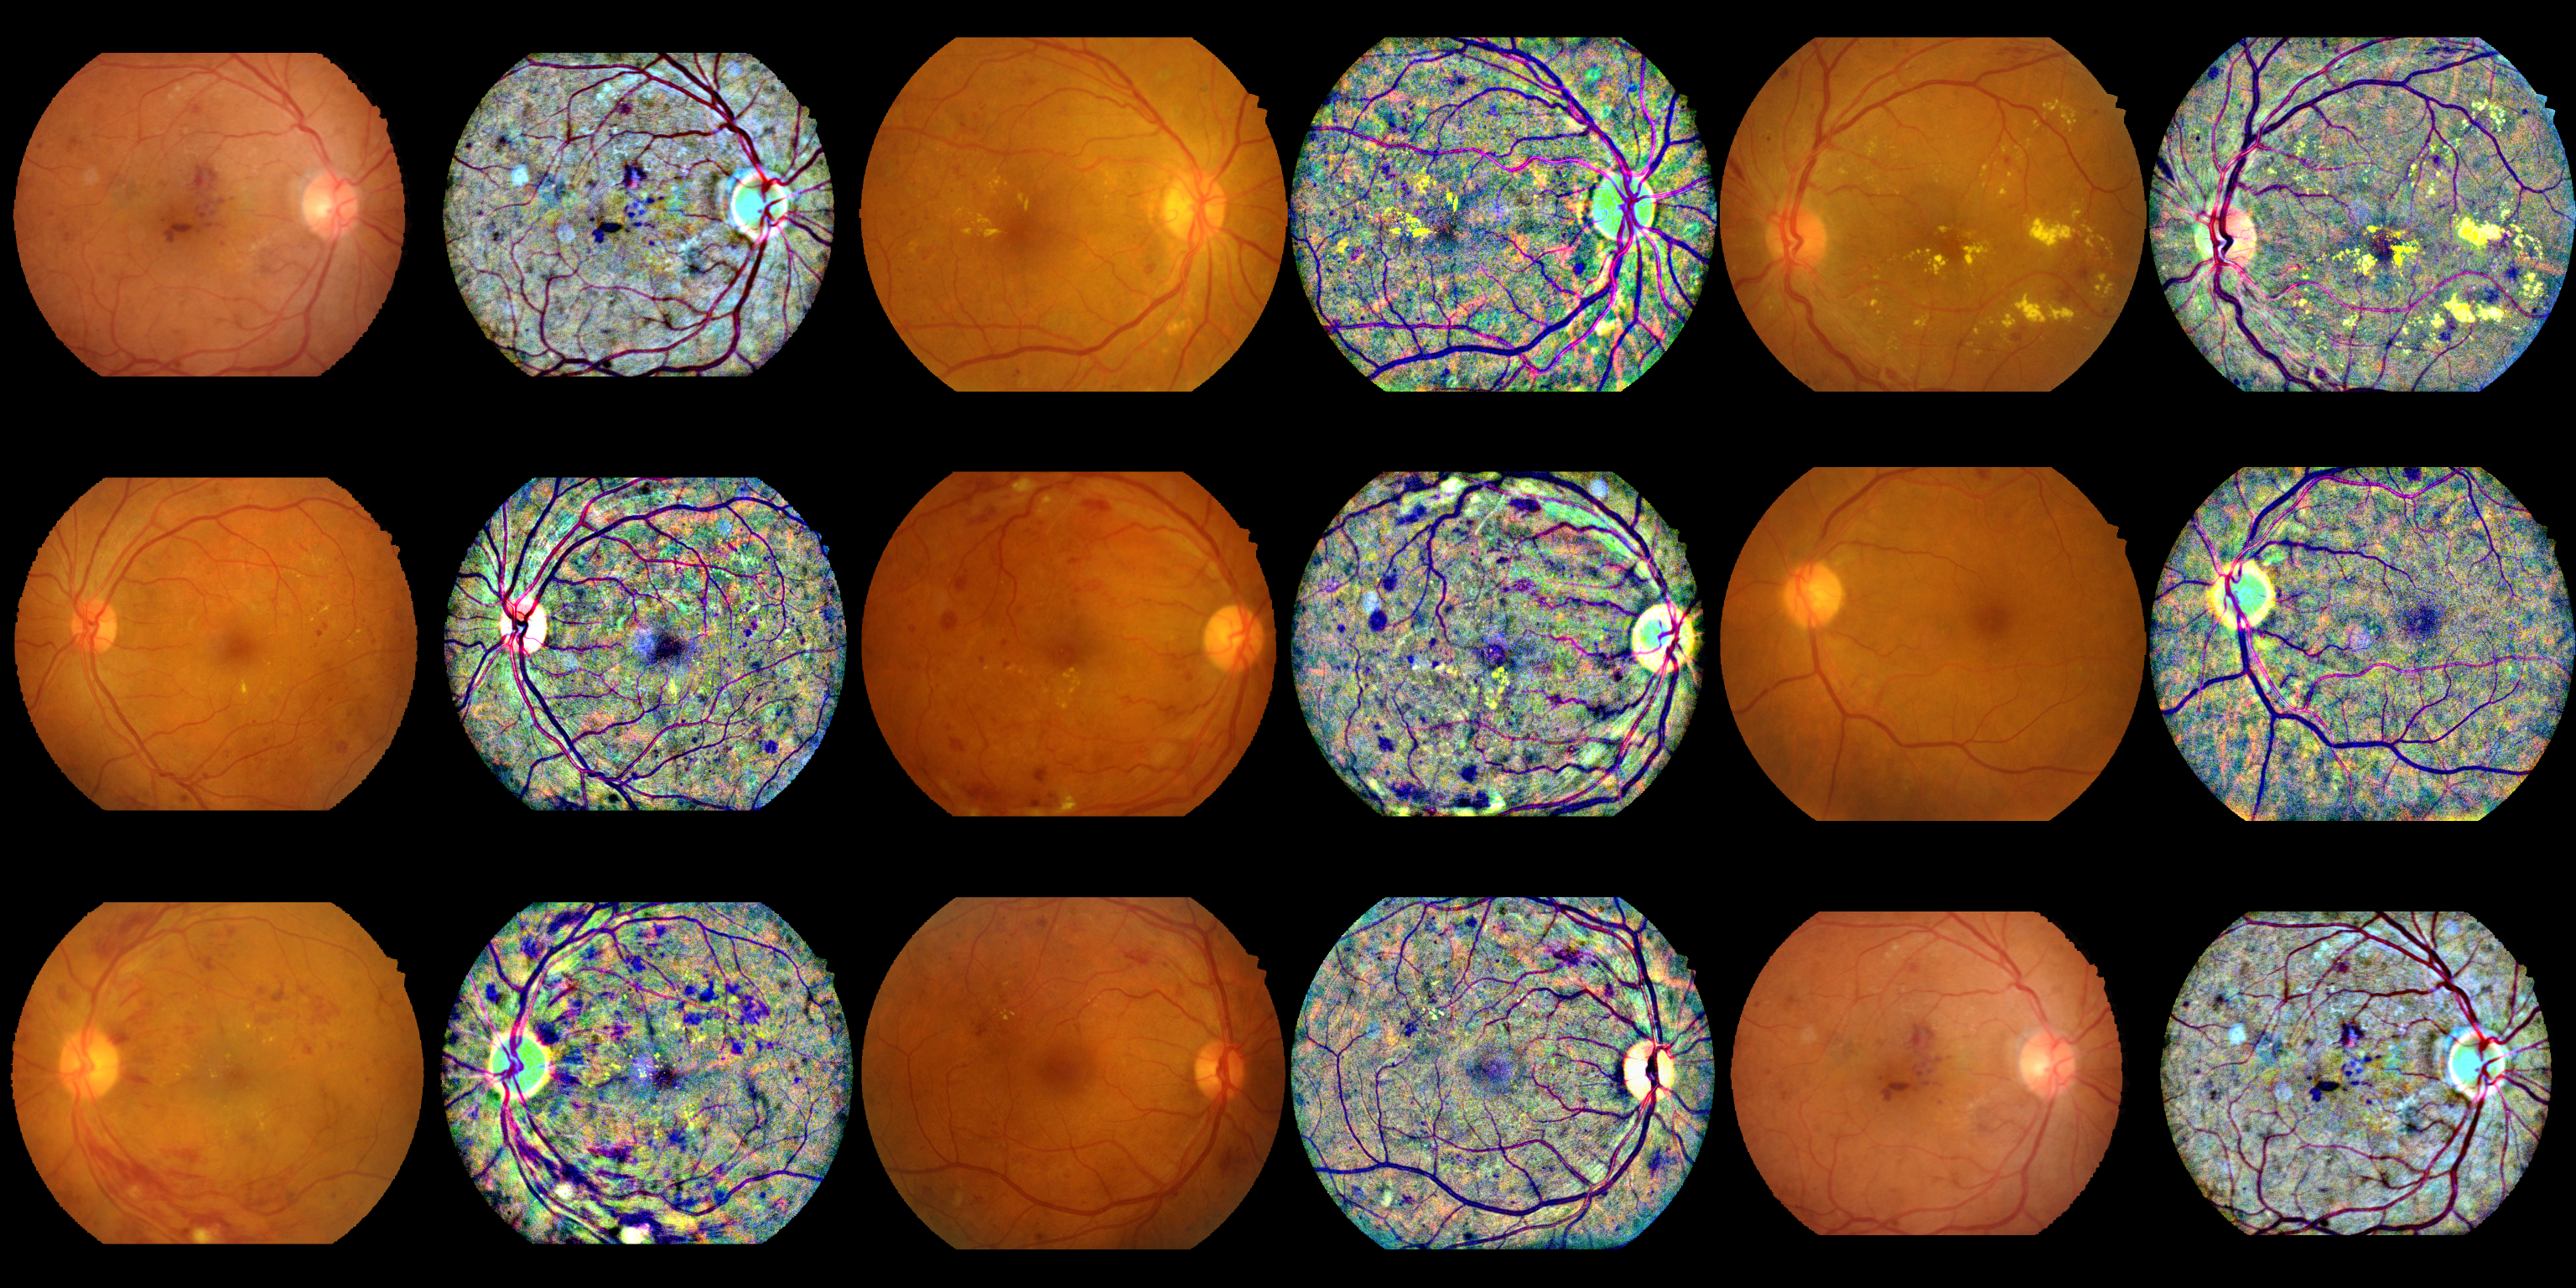
\includegraphics[width=\cellSize\textwidth]{segmentation_lesions/preprocessing_effects/IDRID.png}
		\caption{Entraîné avec IDRID}
	\end{subfigure}
	\begin{subfigure}{\rowSize\textwidth}
		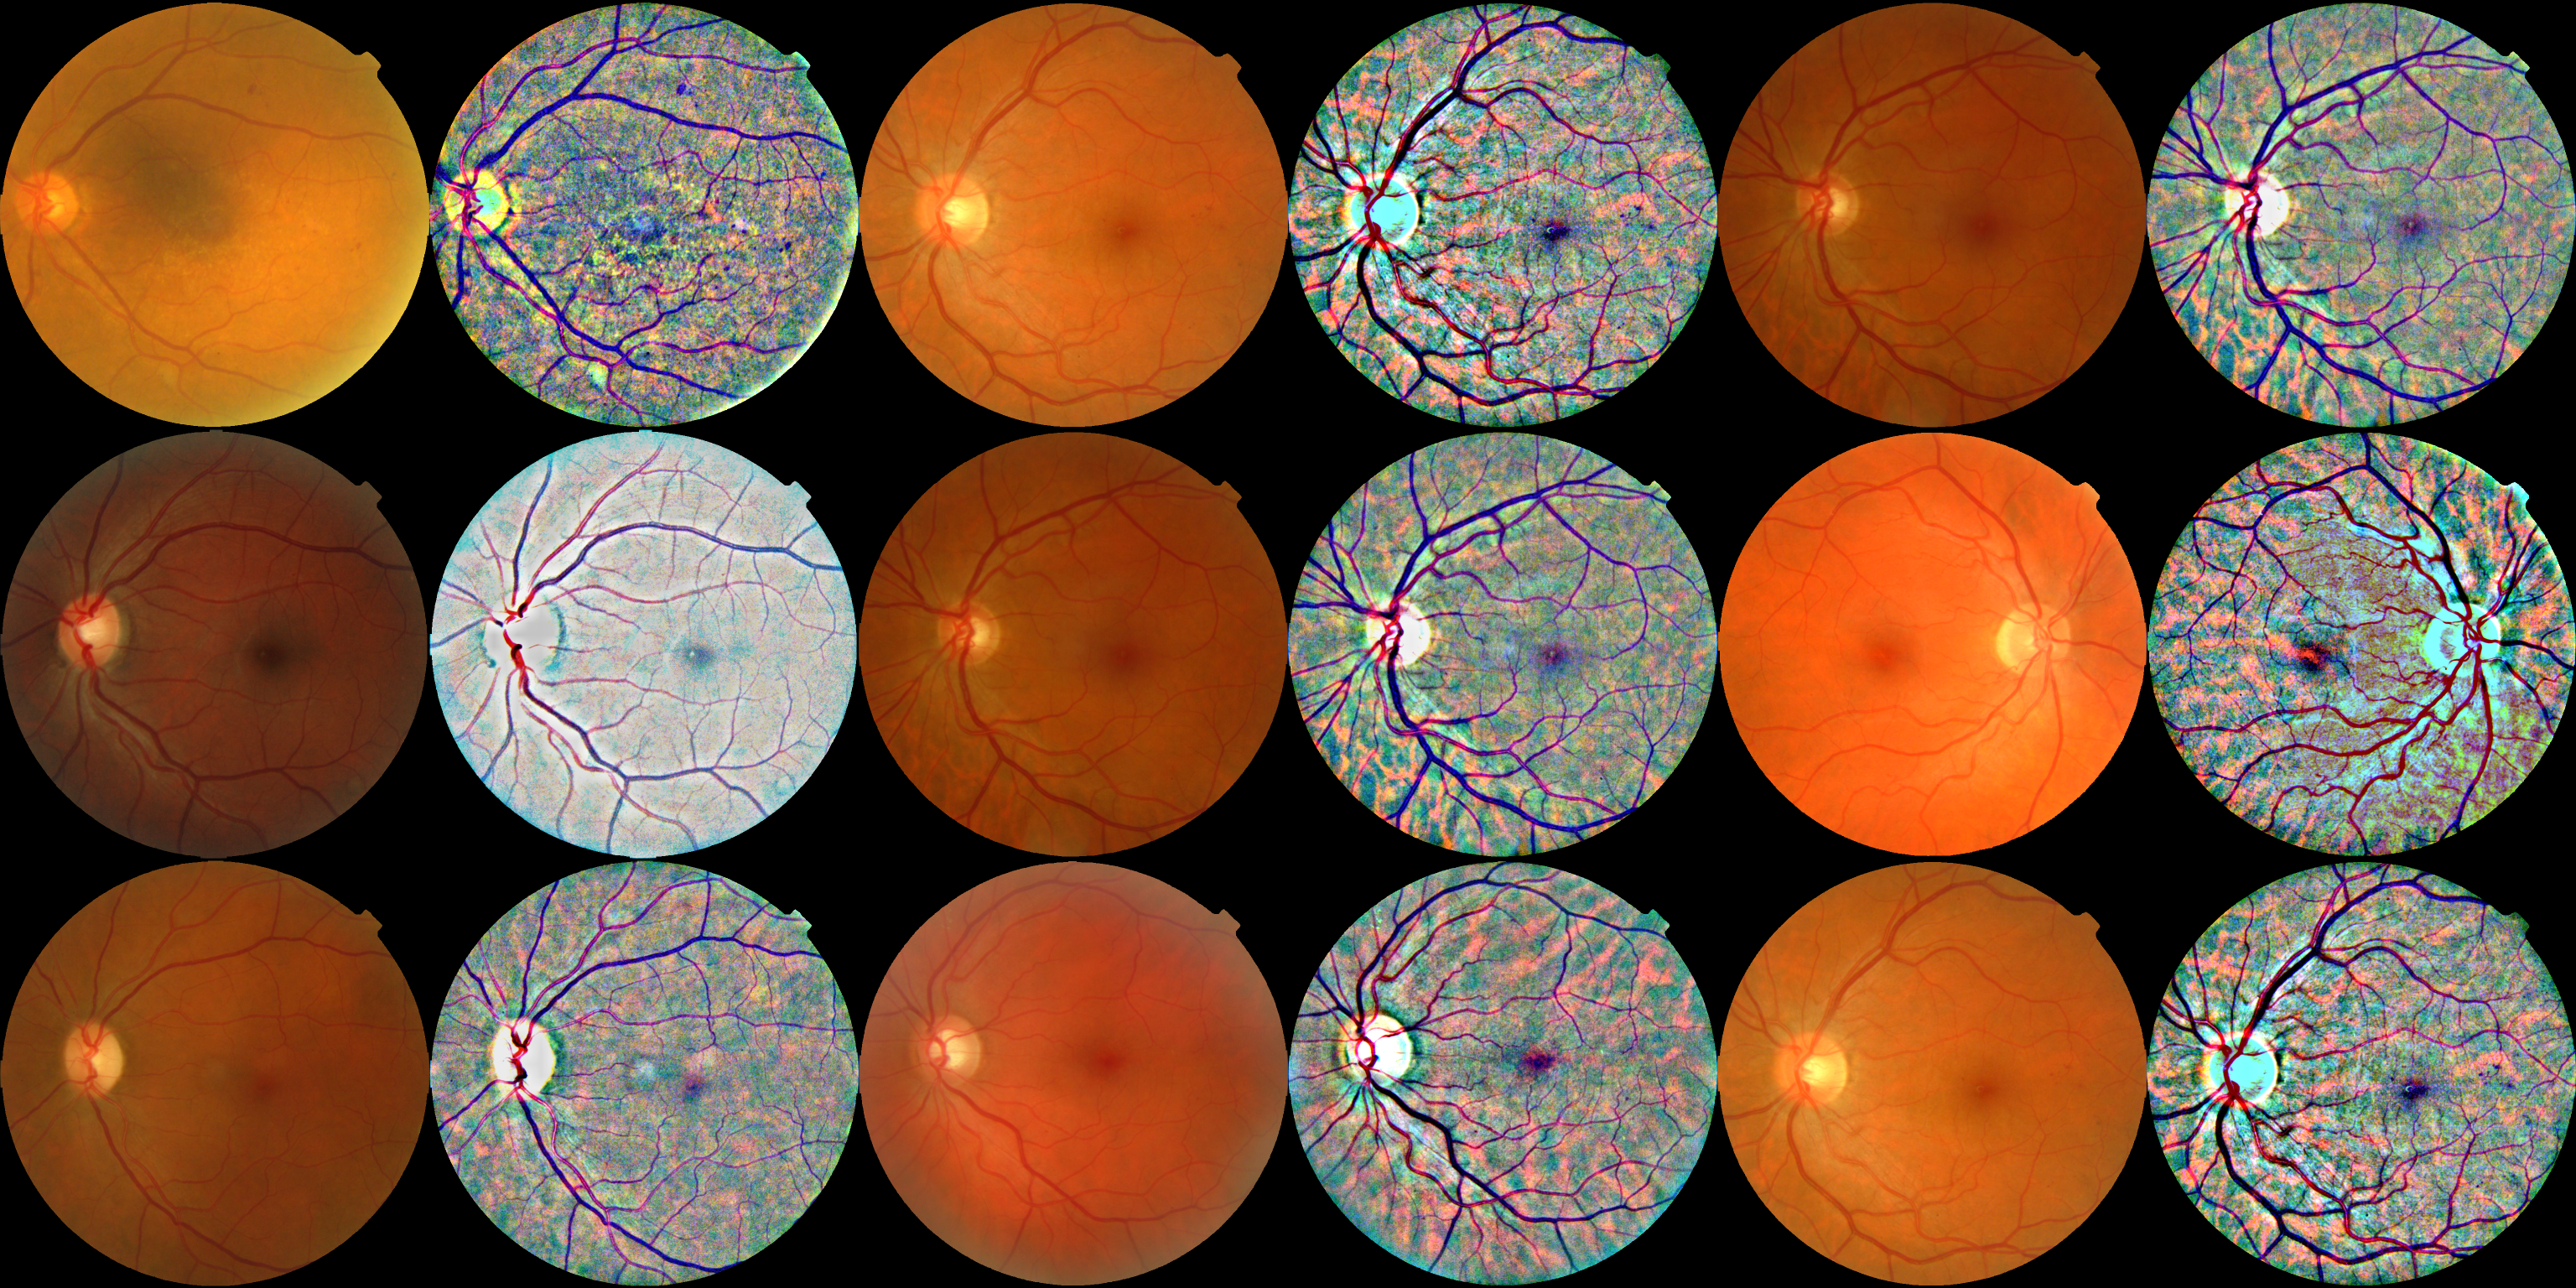
\includegraphics[width=\cellSize\textwidth]{segmentation_lesions/preprocessing_effects/MESSIDOR.png}
		\caption{MESSIDOR}
	\end{subfigure}
	\begin{subfigure}{\rowSize\textwidth}
		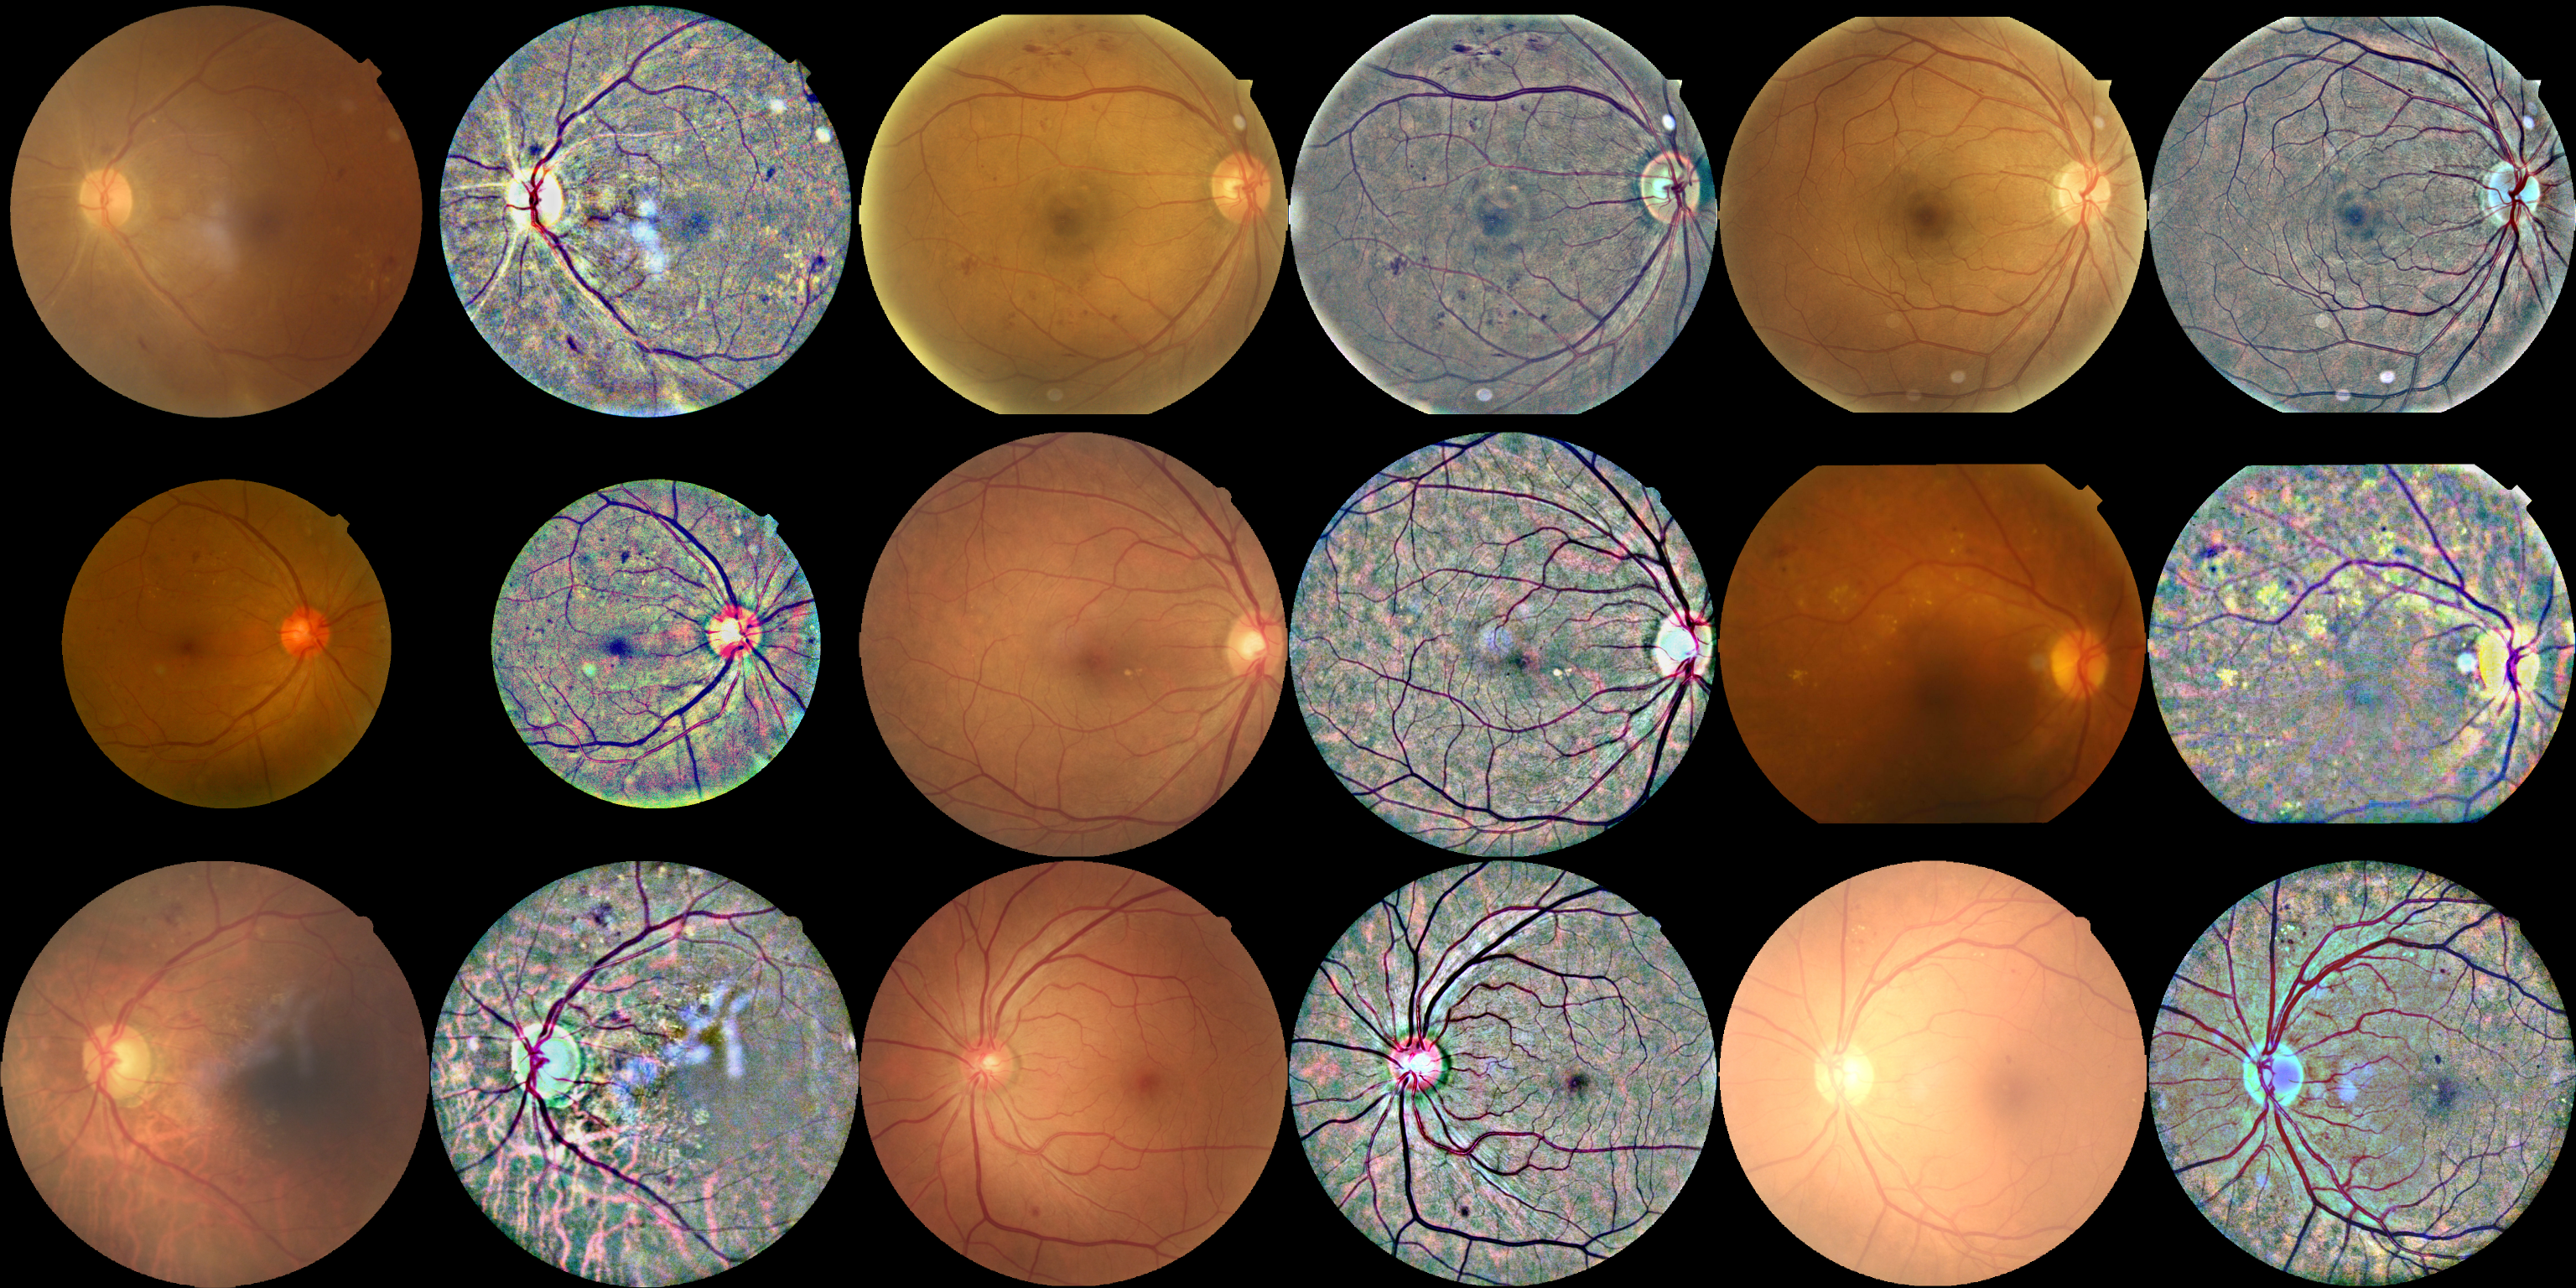
\includegraphics[width=\cellSize\textwidth]{segmentation_lesions/preprocessing_effects/DDR.png}
		\caption{DDR}
	\end{subfigure}
	\begin{subfigure}{\rowSize\textwidth}
		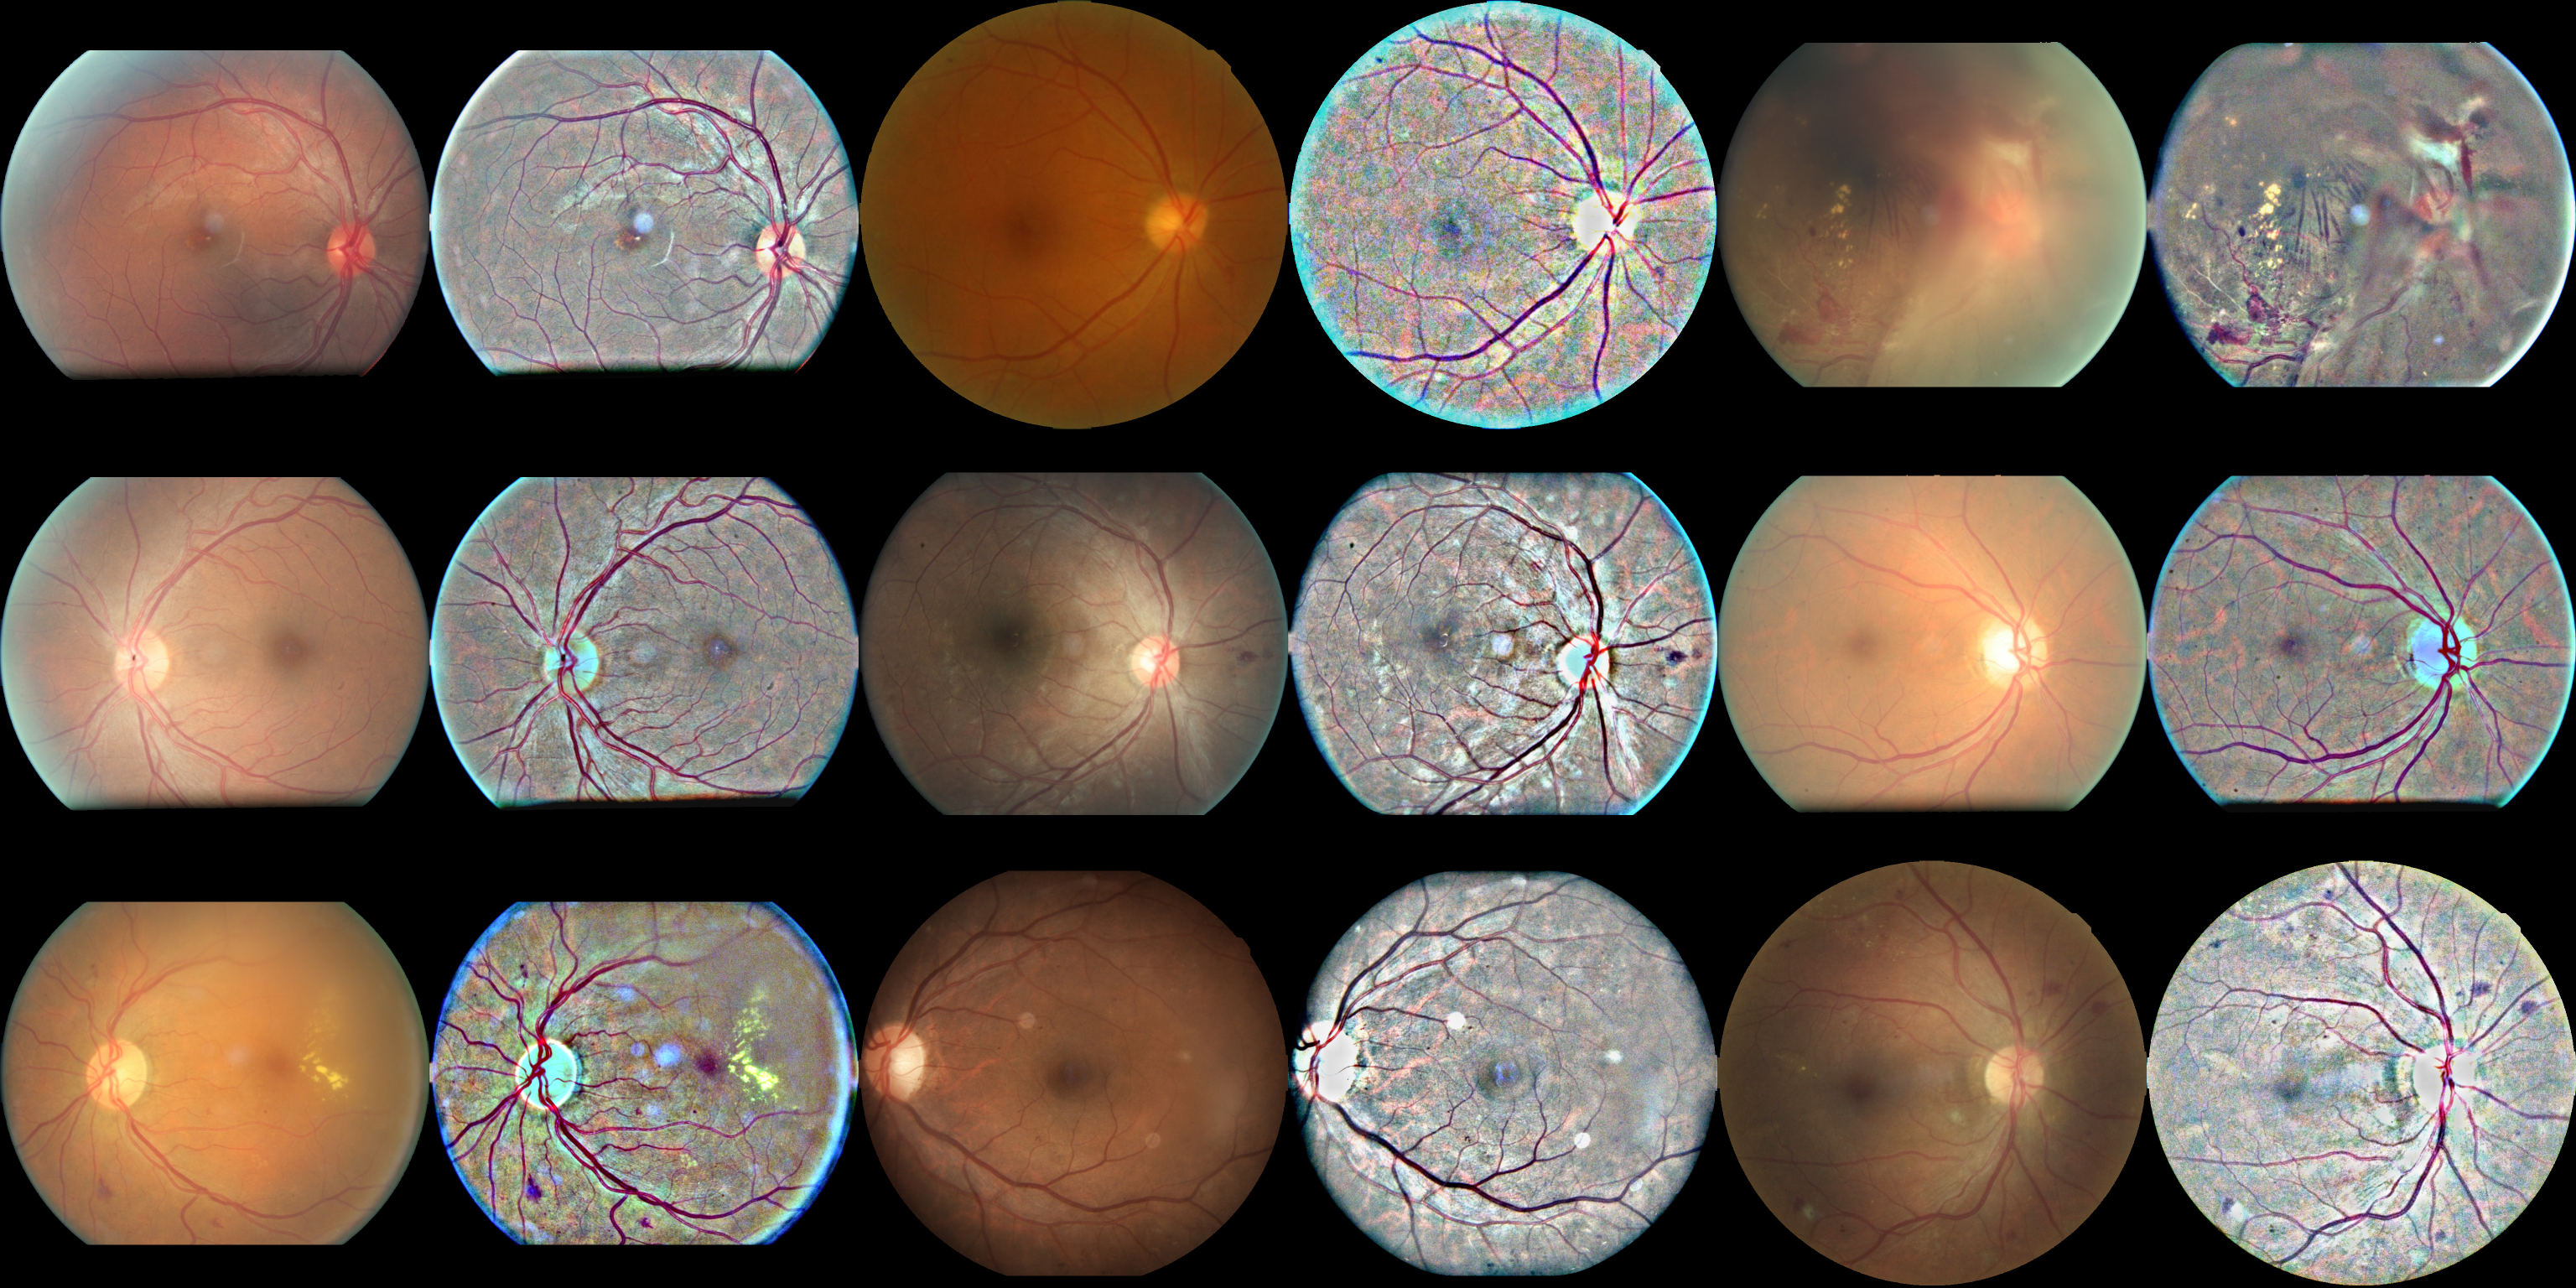
\includegraphics[width=\cellSize\textwidth]{segmentation_lesions/preprocessing_effects/RETINAL_LESIONS.png}
		\caption{RET-LES}
	\end{subfigure}
	\begin{subfigure}{\rowSize\textwidth}
		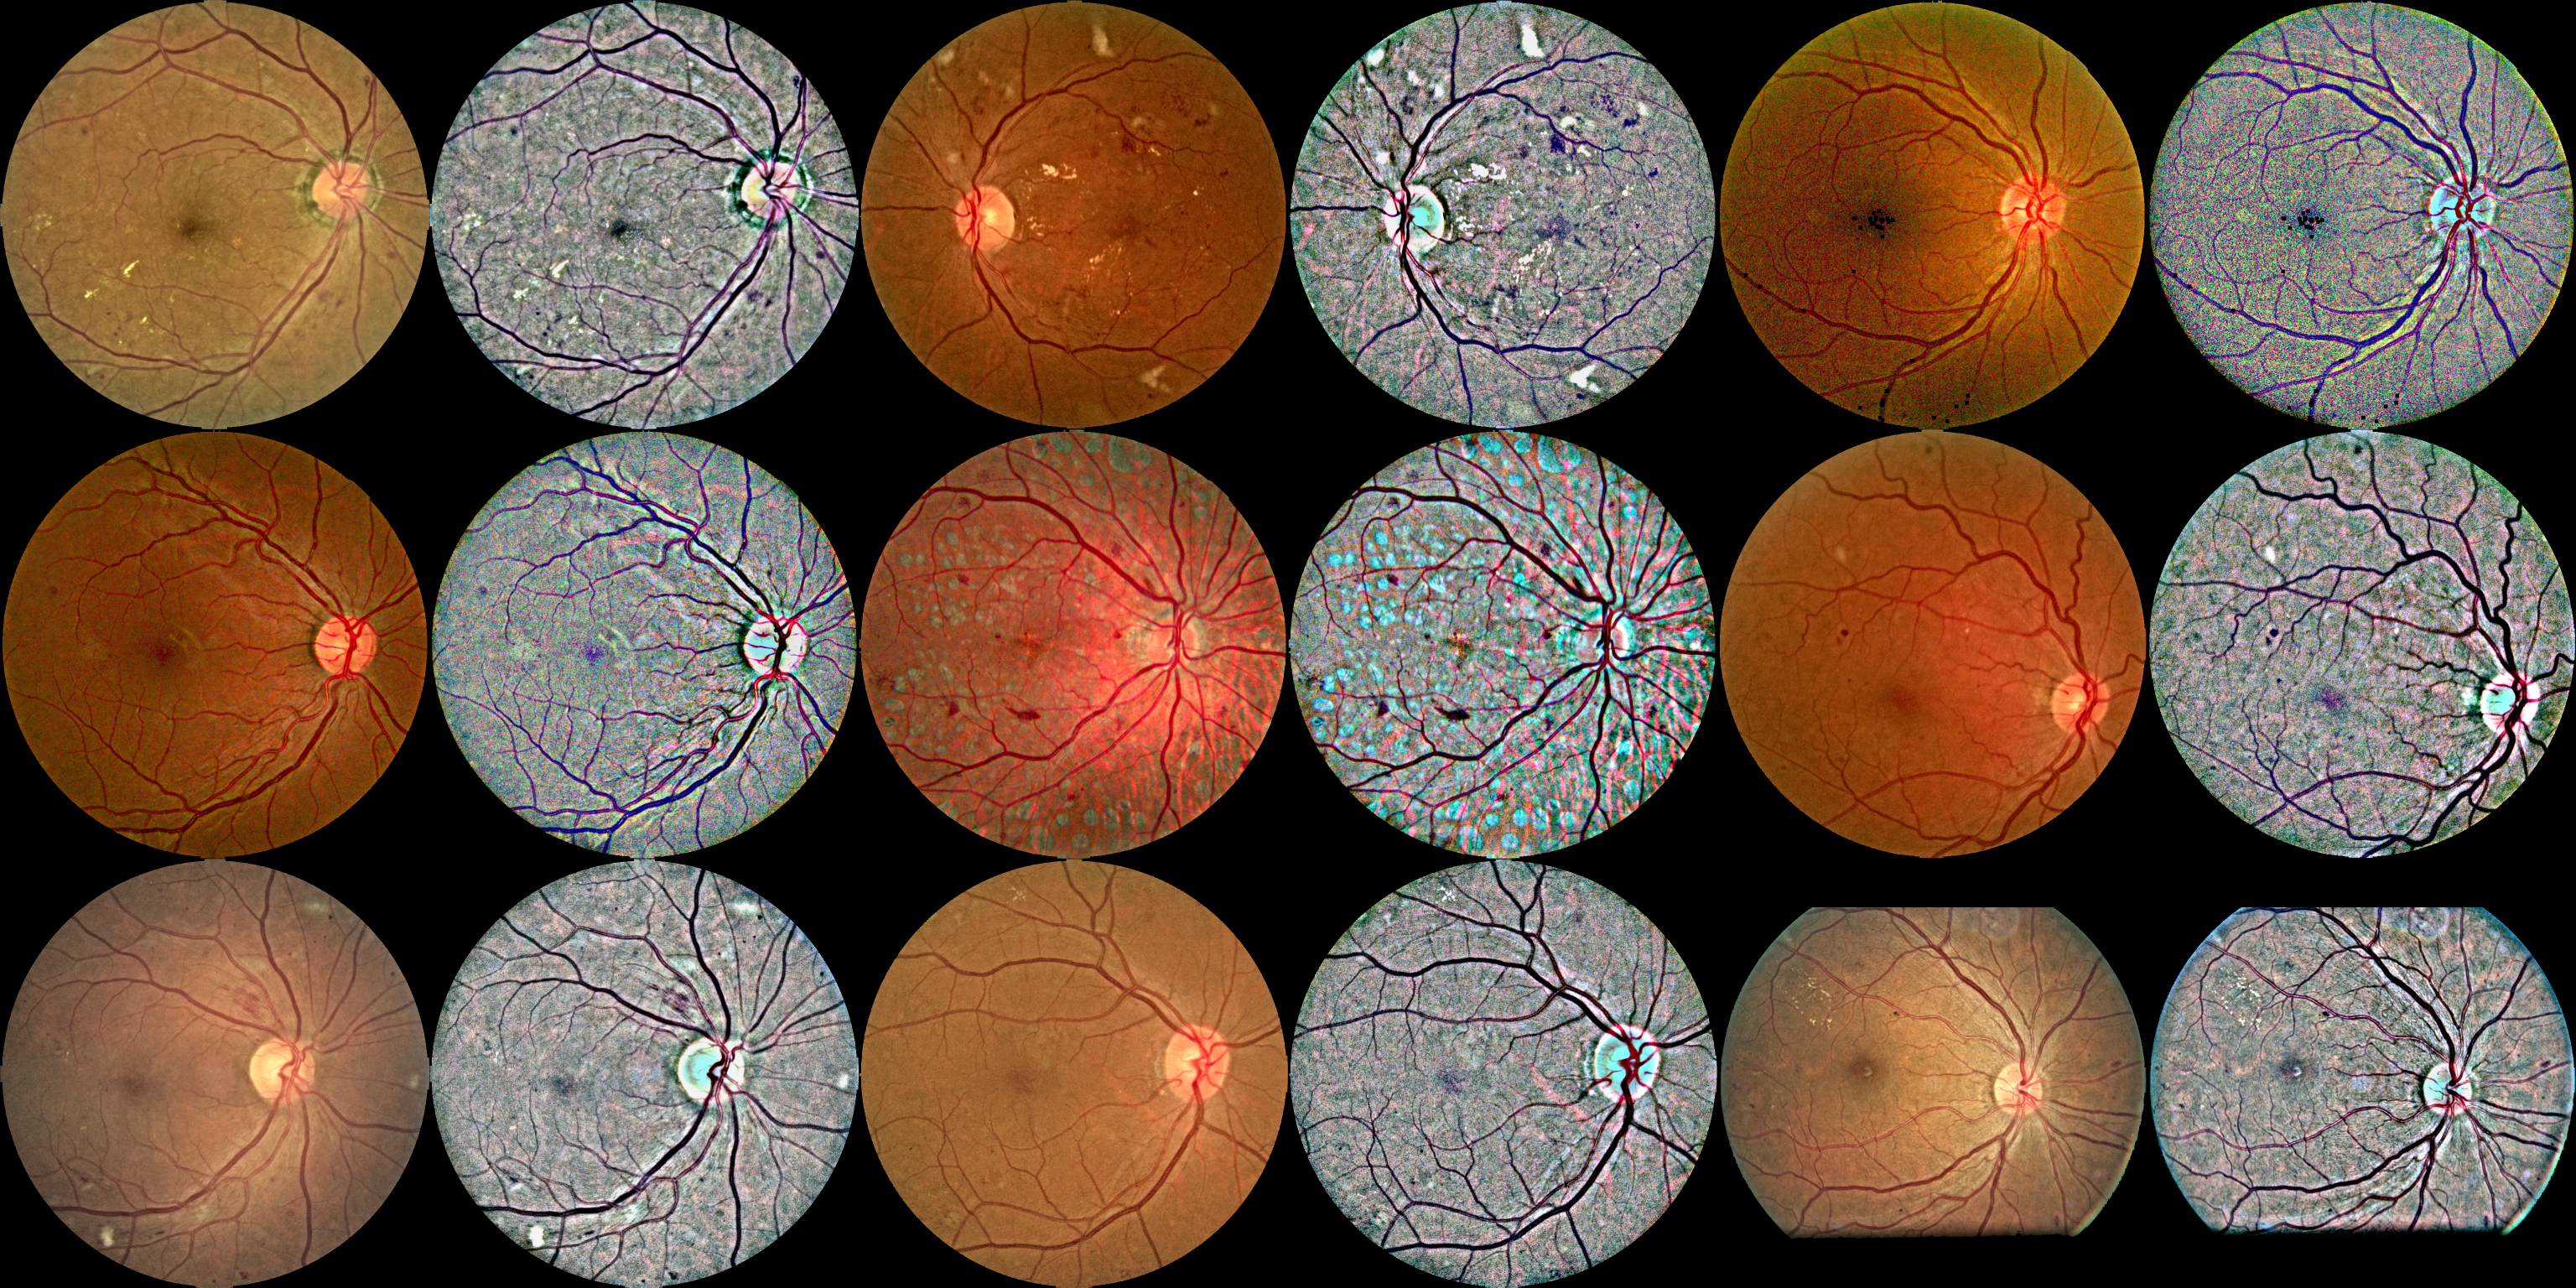
\includegraphics[width=\cellSize\textwidth]{segmentation_lesions/preprocessing_effects/FGADR.png}
		\caption{FGADR}
	\end{subfigure}
	\begin{subfigure}{\rowSize\textwidth}
		\includegraphics[width=\cellSize\textwidth]{segmentation_lesions/preprocessing_effects/ALL.png}
		\caption{En combinant les bases}
	\end{subfigure}
	\caption{Performance (mIoU) comparée avec et sans pré-traitement sur les différents ensemble de test, en fonction de la base d'entraînement}
	\label{fig:preprocessingResultsQuantitave}
\end{figure}


\section{La détection, mesure alternative à la segmentation}
\label{sec:AnnexeDetectionLesions}
Jusqu'à présent, nous avons analysé les modèles à travers leur performance en terme de segmentation sémantique. Les métriques employées pour cela se basent toute sur une analyse pixel-par-pixel: un pixel est soit correctement classifié, soit il ne l'est pas. Or, il existe en réalité une ambiguïté sur la nature de chacun des pixels d'une annotation, ambiguïté qui provient soit d'une interprétation sur la classe d'une structure qui diffère entre les experts-annotateurs, soit d'une appréciation forcément subjective et incertaine des frontières de la structure annotée. Le réseau, entraîné sur une base de donnée, tend à mimer la subjectivité du style d'annotations, notamment en ce qui concerne l'appréciation de la frontière des structures (tel que montré dans la section \ref{sec:SegmentationQualitativeAnalyse}). Cela explique en grande partie les performances de segmentation très variables en fonction de la base sur laquelle le réseau est testé. Or, la forme exacte d'une lésion ne fait pas partie des critères de diagnostic de la maladie sous-jacente (du moins pour la rétinopathie diabétique); l'optimisation de métriques axées sur la segmentation est donc discutable d'un point de vue clinique. Nous proposons en complément une mesure basée sur la détection des lésions en tant que composantes connectées. Pour chaque classe, s'il existe une intersection non vide entre une composante de la prédiction et de l'annotation, alors celle-ci est comptée comme vraie positive. S'il n'y a pas d'intersection, toutes les composantes concernées de l'annotation sont comptées comme fausses négatives; inversement, toutes les composantes de la prédiction sont elles comptées comme fausse positives. 
Ces simples règles sont résumées sur le schéma de la figure \ref{fig:mesuredetection}.
\begin{figure}[H]
	\centering
	\includegraphics[width=0.5\linewidth]{gnuplot/segmentation_lesions/detection/mesureDetection}
	\caption{Règles utilisées pour nos métriques de détection. Les contours pointillés indiquent comment sont interprétées les structures suivant l'intersection de la prédiction et de l'annotation: FP: Faux Positifs (2), FN: Faux Négatifs (1), VP: Vrais Positifs (1)}
	\label{fig:mesuredetection}
\end{figure}
En construisant ainsi une matrice de confusion multiclasses, il est possible de dériver l´équivalent des mesures de sensibilité et de précision, ainsi qu'un score F1, c'est-à-dire la moyenne harmonique des deux. Notons qu'en revanche, en l'absence d'une notion de "Vrai Négatif", il n'est pas possible de mesurer la spécificité. \\
Ces métriques ne peuvent pas remplacer à elles seules l'analyse par segmentation. En effet, dans le cas d'un modèle qui prédirait qu'une prédiction uniforme sur toute l'image (et donc une seule composante connectée), serait considéré comme idéal pour la classe considérée. Il s'agit donc simplement d'un outils d'analyse complémentaire à la segmentation pour comprendre la mécanique des modèles entraînés.
\\
Les résultats sont donnés sur les graphiques de la figure \ref{fig:detectionScore}. On y constate qu'à nouveau, \ac{FGADR} apparaît être la base de données qui pose le plus de problème aux divers modèles. Ainsi, le modèle entraîné sur cette base voit sa sensibilité chuter drastiquement lorsqu'il est testé sur des données issues d'autres bases (indiquant donc en fort nombre de lésions non détectées). L'effet inverse s'observe également lors qu'un modèle est entraîné sur IDRiD ou MESSIDOR (par ailleurs deux bases relativement petites), la précision s´écroule lorsqu'il est testé sur FGADR. Il est intéressant de noter également que le modèle entraîné sur RET-LES, alors qu'il possédait le plus faible mIoU global en terme de segmentation (tableau \ref{tab:generalisationPerfSegmentation}) se révèle être le meilleur modèle en terme de précision et score F1 pour la détection. Cela n'a cependant rien d´étonnant quand on considère que ce modèle segmente peu d'instances et regroupe les lésions en de larges structures peu précises.

\begin{figure}[H]
	\begin{subfigure}{0.495\linewidth}
		\includegraphics[width=\linewidth]{gnuplot/segmentation_lesions/detection/sensitivity}
		\caption{Sensibilité (détection)}
	\end{subfigure}
	\begin{subfigure}{0.495\linewidth}
		\includegraphics[width=\linewidth]{gnuplot/segmentation_lesions/detection/precision}
		\caption{Précision (détection)}
	\end{subfigure}
	\begin{subfigure}{0.495\textwidth}
		\includegraphics[width=\linewidth]{gnuplot/segmentation_lesions/detection/F1}
		\caption{F1 (détection)}
	\end{subfigure}
	\hfill
	\caption{Métriques de détection. Les abscisses représentent les données utilisées pour l'apprentissage.}
	\label{fig:detectionScore}
\end{figure}

\section{Conception d'un modèle de segmentation généraliste}
\label{sec:extendedResultsOnGeneralization}

Au cours de notre expérience sur la généralisation multi-annotations, nous avons expérimenté plusieurs approches pour améliorer les performances du modèle généraliste. Rappelons que la référence que nous utilisons dans nos expériences est $\mathcal{M}_\mathcal{S}=\mathcal{M}[\bigcup_i^T \mathcal{B}^{(i)}]$, c'est-à-dire le modèle simplement entraîné sur la combinaison des bases ($T=\left\lbrace I, M, D, R, F \right\rbrace $). En premier lieu, la combinaison de tous les ensembles peut sembler contre-intuitive, dans la mesure où certains sont plus ou moins \og compatibles \fg entre eux (c'est-à-dire possèdent ou non les mêmes styles d'annotation). Nous nous sommes interrogé sur les sous-ensembles (ou parties) de $T$ qui pourraient être les plus pertinents. Comme $\mathcal{P}(T)  \setminus \emptyset$ (l'ensemble des parties non vides de $T$) est relativement petit ($\text{Card}(\mathcal{P}(T) \setminus \emptyset)  =2^{5}-1 = 31$), il est relativement aisé d'expérimenter avec l'intégralité des combinaisons possibles de base de données. Les résultats sont exposés sur le graphique de la figure \ref{fig:combinaisonPartiesBasesDeDonnees}. On y constate que le meilleur score est bien obtenu par $\mathcal{M}_\mathcal{S}$. La quantité de données prévaut donc sur la qualité de l'homogénéité de celles-ci.
\begin{figure}
	\centering
	\includegraphics[width=\textwidth]{annexe/diceCombinationSets}
	\caption{Performance des différents modèles, entraînés chacun sur une partie de $T$. Les parties sont triées par ordre croissant de cardinalité, c'est-à-dire par le nombre d'images qu'elles contiennent.}
	\label{fig:combinaisonPartiesBasesDeDonnees}
\end{figure}

Au lieu de procéder par la concaténation des images au sein d'une même grande base d'apprentissage, il existe d'autres façons de combiner les données. Nous en avons expérimenté deux:
\begin{itemize}
	\item L'entraînement d'un modèle par base de données suivi de la moyenne des prédictions réalisées par chaque modèle à l'inférence. Cette stratégie est appelée \og Ensemble de Modèles \fg.
	\item Similairement, l'entraînement d'un modèle par base de données, mais cette fois, la moyenne des poids de chaque modèle est réalisé à l'inférence. Cette idée est empruntée à Wortsman et al. \cite{wortsman2022model} qui la nomme \og Soupe de Modèles \fg.
\end{itemize}
Notons que dans un cas comme dans l'autre, il suffit de n'entraîner que cinq modèles ($\mathcal{M}[\mathcal{B}^{(I)}]$, $\mathcal{M}[\mathcal{B}^{(M)}]$, $\mathcal{M}[\mathcal{B}^{(D)}]$, $\mathcal{M}[\mathcal{B}^{(R)}]$ et $ \mathcal{M}[\mathcal{B}^{(F)}]$), qui seront ensuite combinés aux besoins. À nouveau, 31 combinaisons sont possibles. Précisons cependant que la technique de Wortsman et al. est très récente et n'a été appliquée que sur des réseaux de classification. Pour la segmentation, nous n'avons obtenu de résultats fonctionnels qu'en limitant les \og soupes \fg aux poids de l'encodeur. Pour chacune de celles-ci, 5 décodeurs peuvent donc être adoptés, créant donc $5 \times 31 = 155$ modèles possibles au total. En pratique, dans nos expériences, nous nous sommes limités qu'à 31 modèles (soupe d'encodeurs et décodeur issu de $\mathcal{M}_\mathcal{S}$). Les résultats obtenus avec les différentes techniques sont donnés sur la figure \ref{fig:GeneralizationResultsSoupEnsembleCombination}. Il y apparaît clairement que la concaténation des données d'entraînement est la plus efficace des trois stratégies, quelle que soit la combinaison empruntée.
\begin{figure}
	\centering
	\includegraphics[width=\textwidth]{annexe/generalization_methods}
	\caption{Résultats de différentes méthodes de combinaisons des bases de données. Seul le Dice moyen est fourni ($\frac{1}{5} \sum_{i=1}^{5}$ $D(\mathcal{M}, \mathcal{B}^{(i)}_\star)$). L'écart-type est représenté en pointillés ($\pm \sigma$).}
	\label{fig:GeneralizationResultsSoupEnsembleCombination}
\end{figure}
Nous avons mené d'autres expériences dans le but de combiner différemment les modèles, mais nos efforts en ce sens se sont révélés infructueux (absence de convergence ou performances très en deçà de celles obtenues avec les modèles classiques). En vrac, citons:
\begin{itemize}
	\item L'adaptation adversarial par un système à double générateurs (GAN): le premier GAN est chargé de modifier le style de chaque image d'entrée vers un domaine cible (en l'occurence $\mathcal{B}^{(I)}$). Le second GAN a pour objectif de modifier le style d'annotation vers celui du domaine cible, là encore $\mathcal{B}^{(I)}$. Entre ces deux GAN, un réseau de segmentation classique manipule les images et les annotations adversarialement converties par chaque GAN. 
	\item La régularisation par apprentissage auto-entraîné (\textit{self training}), en exploitant une large base de données non-labellisées. Un premier réseau est entraîné sur $\mathcal{B}^{(I)}$, fait de l'inférence sur une grande base d'image (EyePACS). Ses prédictions servent à entraîner un second réseau, conjointement avec $\mathcal{B}^{(I)}$. Nous n'avons pas obtenu d'améliorations par l'ajout des images auto-annotées.
	\item La régularisation par apprentissage contrastif (\textit{Contrastive Learning}) en ré-implémentant l'approche de Zhao et al. \cite{zhaoContrastiveLearningLabel2021}. Nous n'avons pas réussi à faire converger ce modèle.
\end{itemize}
Même sans rentrer dans les détails, c'est différentes expérimentations illustrent le potentiel de sophistication de la segmentation sémantique du \fundus{}. Chacune de ces expériences est théoriquement fondée; malheureusement en pratique, nous nous sommes heurté à la difficulté de les faire converger adéquatement, y compris en tentant de respecter scrupuleusement les méthodologies existantes. Si cela nous confronte à la difficulté de la reproductibilité de la littérature, il n'est pas exclu que des efforts plus conséquents dans une voie donnée pourraient mener à des résultats bien plus aboutis.
